% **************************************************************************************************************

% A Classic Thesis Style
% An Homage to The Elements of Typographic Style
%
% Copyright (C) 2015 André Miede http://www.miede.de
%
% If you like the style then I would appreciate a postcard. My address
% can be found in the file ClassicThesis.pdf. A collection of the
% postcards I received so far is available online at
% http://postcards.miede.de
%
% License:
% This program is free software; you can redistribute it and/or modify
% it under the terms of the GNU General Public License as published by
% the Free Software Foundation; either version 2 of the License, or
% (at your option) any later version.
%
% This program is distributed in the hope that it will be useful,
% but WITHOUT ANY WARRANTY; without even the implied warranty of
% MERCHANTABILITY or FITNESS FOR A PARTICULAR PURPOSE.  See the
% GNU General Public License for more details.
%
% You should have received a copy of the GNU General Public License
% along with this program; see the file COPYING.  If not, write to
% the Free Software Foundation, Inc., 59 Temple Place - Suite 330,
% Boston, MA 02111-1307, USA.
%
% **************************************************************************************************************
\RequirePackage{fix-cm} % fix some latex issues see: http://texdoc.net/texmf-dist/doc/latex/base/fixltx2e.pdf
\documentclass[ oneside,openright,titlepage,numbers=noenddot,headinclude,%1headlines,% letterpaper a4paper
                footinclude=true,cleardoublepage=empty,abstract=false, % <--- obsolete, remove (todo)
                %BCOR=5mm, % for binding with twosided
                %DIV=12, % increase to decrease blank on the sides
                paper=a4,fontsize=11pt,%11pt,a4paper,%
                ngerman,american,%
                ]{scrreprt}
%********************************************************************
% Note: Make all your adjustments in here
%*******************************************************
% ****************************************************************************************************
% classicthesis-config.tex
% formerly known as loadpackages.sty, classicthesis-ldpkg.sty, and classicthesis-preamble.sty
% Use it at the beginning of your ClassicThesis.tex, or as a LaTeX Preamble
% in your ClassicThesis.{tex,lyx} with % ****************************************************************************************************
% classicthesis-config.tex
% formerly known as loadpackages.sty, classicthesis-ldpkg.sty, and classicthesis-preamble.sty
% Use it at the beginning of your ClassicThesis.tex, or as a LaTeX Preamble
% in your ClassicThesis.{tex,lyx} with % ****************************************************************************************************
% classicthesis-config.tex
% formerly known as loadpackages.sty, classicthesis-ldpkg.sty, and classicthesis-preamble.sty
% Use it at the beginning of your ClassicThesis.tex, or as a LaTeX Preamble
% in your ClassicThesis.{tex,lyx} with \input{classicthesis-config}
% ****************************************************************************************************
% If you like the classicthesis, then I would appreciate a postcard.
% My address can be found in the file ClassicThesis.pdf. A collection
% of the postcards I received so far is available online at
% http://postcards.miede.de
% ****************************************************************************************************
%packages added by Anran

\usepackage{amssymb}
\usepackage{amsthm} % for theorem environment
\usepackage{dsfont}
\usepackage{stmaryrd}
\usepackage{controlSequences}
\usepackage{comment}
\usepackage{hhline}
\usepackage{ebproof} % typesetting inference rules 
%\usepackage{framed} % to use leftbar

% ****************************************************************************************************
% 0. Set the encoding of your files. UTF-8 is the only sensible encoding nowadays. If you can't read
% äöüßáéçèê∂åëæƒÏ€ then change the encoding setting in your editor, not the line below. If your editor
% does not support utf8 use another editor!
% ****************************************************************************************************
\PassOptionsToPackage{utf8}{inputenc}
	\usepackage{inputenc}

% ****************************************************************************************************
% 1. Configure classicthesis for your needs here, e.g., remove "drafting" below
% in order to deactivate the time-stamp on the pages
% ****************************************************************************************************
\PassOptionsToPackage{eulerchapternumbers,listings,%drafting,%
					 pdfspacing,%floatperchapter,%linedheaders,%
					 subfig,beramono,eulermath,parts}{classicthesis}
% ********************************************************************
% Available options for classicthesis.sty
% (see ClassicThesis.pdf for more information):
% drafting
% parts nochapters linedheaders
% eulerchapternumbers beramono eulermath pdfspacing minionprospacing
% tocaligned dottedtoc manychapters
% listings floatperchapter subfig
% ********************************************************************


% ****************************************************************************************************
% 2. Personal data and user ad-hoc commands
% ****************************************************************************************************
\newcommand{\myTitle}{Necessary Liberal Preconditions: A Proof System\xspace}
\newcommand{\myTitleDe}{Notwendige Liberale Vorbedingungen: Ein Beweissystem\xspace}
%\newcommand{\mySubtitle}{\xspace}
\newcommand{\myType}{Mster's Thesis in Informatics\xspace}
\newcommand{\myDegree}{B.Sc.\xspace}
\newcommand{\myName}{Anran Wang\xspace}
\newcommand{\myProf}{Prof. Jan Křetínský\xspace}
\newcommand{\myOtherProf}{Prof. Benjamin Lucien Kaminski\xspace}
\newcommand{\mySupervisor}{Lena Verscht, M.Sc.\xspace}
%\newcommand{\myFaculty}{Put data here\xspace}
\newcommand{\myDepartment}{School of Computation, Information and Technology - Informatics\xspace}
\newcommand{\myUni}{Technical University of Munich\xspace}
\newcommand{\myLocation}{Munich\xspace}
\newcommand{\myTime}{March 2023\xspace}
\newcommand{\myVersion}{version 0.1\xspace}

% ********************************************************************
% Setup, finetuning, and useful commands
% ********************************************************************
\newcounter{dummy} % necessary for correct hyperlinks (to index, bib, etc.)
\newlength{\abcd} % for ab..z string length calculation
\providecommand{\mLyX}{L\kern-.1667em\lower.25em\hbox{Y}\kern-.125emX\@}
\newcommand{\ie}{i.\,e.}
\newcommand{\Ie}{I.\,e.}
\newcommand{\eg}{e.\,g.}
\newcommand{\Eg}{E.\,g.}
% ****************************************************************************************************

% ****************************************************************************************************
% 3. Loading some handy packages
% ****************************************************************************************************
% ********************************************************************
% Packages with options that might require adjustments
% ********************************************************************
%\PassOptionsToPackage{ngerman,american}{babel}   % change this to your language(s)
% Spanish languages need extra options in order to work with this template
%\PassOptionsToPackage{spanish,es-lcroman}{babel}
	\usepackage{babel}

\usepackage{csquotes}
\PassOptionsToPackage{%
    %backend=biber, %instead of bibtex
	backend=bibtex8,bibencoding=ascii,%
	language=auto,%
	style=numeric-comp,%
    %style=authoryear-comp, % Author 1999, 2010
    %bibstyle=authoryear,dashed=false, % dashed: substitute rep. author with ---
    sorting=nyt, % name, year, title
    maxbibnames=10, % default: 3, et al.
    %backref=true,%
    natbib=true % natbib compatibility mode (\citep and \citet still work)
}{biblatex}
    \usepackage{biblatex}

\PassOptionsToPackage{fleqn}{amsmath}       % math environments and more by the AMS
    \usepackage{amsmath}

% ********************************************************************
% General useful packages
% ********************************************************************
\PassOptionsToPackage{T1}{fontenc} % T2A for cyrillics
    \usepackage{fontenc}
\usepackage{textcomp} % fix warning with missing font shapes
\usepackage{scrhack} % fix warnings when using KOMA with listings package
\usepackage{xspace} % to get the spacing after macros right
\usepackage{mparhack} % get marginpar right
\usepackage{fixltx2e} % fixes some LaTeX stuff --> since 2015 in the LaTeX kernel (see below)
%\usepackage[latest]{latexrelease} % will be used once available in more distributions (ISSUE #107)
\PassOptionsToPackage{printonlyused,smaller}{acronym}
    \usepackage{acronym} % nice macros for handling all acronyms in the thesis
    %\renewcommand{\bflabel}[1]{{#1}\hfill} % fix the list of acronyms --> no longer working
    %\renewcommand*{\acsfont}[1]{\textsc{#1}}
    \renewcommand*{\aclabelfont}[1]{\acsfont{#1}}
% ****************************************************************************************************


% ****************************************************************************************************
% 4. Setup floats: tables, (sub)figures, and captions
% ****************************************************************************************************
\usepackage{tabularx} % better tables
    \setlength{\extrarowheight}{3pt} % increase table row height
\newcommand{\tableheadline}[1]{\multicolumn{1}{c}{\spacedlowsmallcaps{#1}}}
\newcommand{\myfloatalign}{\centering} % to be used with each float for alignment
\usepackage{caption}
% Thanks to cgnieder and Claus Lahiri
% http://tex.stackexchange.com/questions/69349/spacedlowsmallcaps-in-caption-label
% [REMOVED DUE TO OTHER PROBLEMS, SEE ISSUE #82]
%\DeclareCaptionLabelFormat{smallcaps}{\bothIfFirst{#1}{~}\MakeTextLowercase{\textsc{#2}}}
%\captionsetup{font=small,labelformat=smallcaps} % format=hang,
\captionsetup{font=small} % format=hang,
\usepackage{subfig}
% ****************************************************************************************************


% ****************************************************************************************************
% 5. Setup code listings
% ****************************************************************************************************
\usepackage{listings}
%\lstset{emph={trueIndex,root},emphstyle=\color{BlueViolet}}%\underbar} % for special keywords
\lstset{language=[LaTeX]Tex,%C++,
    morekeywords={PassOptionsToPackage,selectlanguage},
    keywordstyle=\color{RoyalBlue},%\bfseries,
    basicstyle=\small\ttfamily,
    %identifierstyle=\color{NavyBlue},
    commentstyle=\color{Green}\ttfamily,
    stringstyle=\rmfamily,
    numbers=none,%left,%
    numberstyle=\scriptsize,%\tiny
    stepnumber=5,
    numbersep=8pt,
    showstringspaces=false,
    breaklines=true,
    %frameround=ftff,
    %frame=single,
    belowcaptionskip=.75\baselineskip
    %frame=L
}
% ****************************************************************************************************


% ****************************************************************************************************
% 6. PDFLaTeX, hyperreferences and citation backreferences
% ****************************************************************************************************
% ********************************************************************
% Using PDFLaTeX
% ********************************************************************
\PassOptionsToPackage{pdftex,hyperfootnotes=false,pdfpagelabels}{hyperref}
    \usepackage{hyperref}  % backref linktocpage pagebackref
\pdfcompresslevel=9
\pdfadjustspacing=1
\PassOptionsToPackage{pdftex}{graphicx}
    \usepackage{graphicx}


% ********************************************************************
% Hyperreferences
% ********************************************************************
\hypersetup{%
    %draft, % = no hyperlinking at all (useful in b/w printouts)
    colorlinks=true, linktocpage=true, pdfstartpage=3, pdfstartview=FitV,%
    % uncomment the following line if you want to have black links (e.g., for printing)
    %colorlinks=false, linktocpage=false, pdfstartpage=3, pdfstartview=FitV, pdfborder={0 0 0},%
    breaklinks=true, pdfpagemode=UseNone, pageanchor=true, pdfpagemode=UseOutlines,%
    plainpages=false, bookmarksnumbered, bookmarksopen=true, bookmarksopenlevel=1,%
    hypertexnames=true, pdfhighlight=/O,%nesting=true,%frenchlinks,%
    urlcolor=webbrown, linkcolor=RoyalBlue, citecolor=webgreen, %pagecolor=RoyalBlue,%
    %urlcolor=Black, linkcolor=Black, citecolor=Black, %pagecolor=Black,%
    pdftitle={\myTitle},%
    pdfauthor={\textcopyright\ \myName, \myUni, \myDepartment},%
    pdfsubject={},%
    pdfkeywords={},%
    pdfcreator={pdfLaTeX},%
    pdfproducer={LaTeX with hyperref and classicthesis}%
}

% ********************************************************************
% Setup autoreferences
% ********************************************************************
% There are some issues regarding autorefnames
% http://www.ureader.de/msg/136221647.aspx
% http://www.tex.ac.uk/cgi-bin/texfaq2html?label=latexwords
% you have to redefine the makros for the
% language you use, e.g., american, ngerman
% (as chosen when loading babel/AtBeginDocument)
% ********************************************************************
\makeatletter
\@ifpackageloaded{babel}%
    {%
       \addto\extrasamerican{%
			\renewcommand*{\figureautorefname}{Figure}%
			\renewcommand*{\tableautorefname}{Table}%
			\renewcommand*{\partautorefname}{Part}%
			\renewcommand*{\chapterautorefname}{Chapter}%
			\renewcommand*{\sectionautorefname}{Section}%
			\renewcommand*{\subsectionautorefname}{Section}%
            \renewcommand*{\subsubsectionautorefname}{Section}%
                }%
       \addto\extrasngerman{%
			\renewcommand*{\paragraphautorefname}{Absatz}%
			\renewcommand*{\subparagraphautorefname}{Unterabsatz}%
			\renewcommand*{\footnoteautorefname}{Fu\"snote}%
			\renewcommand*{\FancyVerbLineautorefname}{Zeile}%
			\renewcommand*{\theoremautorefname}{Theorem}%
			\renewcommand*{\appendixautorefname}{Anhang}%
			\renewcommand*{\equationautorefname}{Gleichung}%
			\renewcommand*{\itemautorefname}{Punkt}%
                }%
            % Fix to getting autorefs for subfigures right (thanks to Belinda Vogt for changing the definition)
            \providecommand{\subfigureautorefname}{\figureautorefname}%
    }{\relax}
\makeatother


% ****************************************************************************************************
% 7. Last calls before the bar closes
% ****************************************************************************************************
% ********************************************************************
% Development Stuff
% ********************************************************************
\listfiles
%\PassOptionsToPackage{l2tabu,orthodox,abort}{nag}
%   \usepackage{nag}
%\PassOptionsToPackage{warning, all}{onlyamsmath}
%   \usepackage{onlyamsmath}

% ********************************************************************
% Last, but not least...
% ********************************************************************
\usepackage{classicthesis}
% ****************************************************************************************************


% ****************************************************************************************************
% 8. Further adjustments (experimental)
% ****************************************************************************************************
% ********************************************************************
% Changing the text area
% ********************************************************************
%\linespread{1.05} % a bit more for Palatino
%\areaset[current]{312pt}{761pt} % 686 (factor 2.2) + 33 head + 42 head \the\footskip
%\setlength{\marginparwidth}{7em}%
%\setlength{\marginparsep}{2em}%

% ********************************************************************
% Using different fonts
% ********************************************************************
%\usepackage[oldstylenums]{kpfonts} % oldstyle notextcomp
%\usepackage[osf]{libertine}
%\usepackage[light,condensed,math]{iwona}
%\renewcommand{\sfdefault}{iwona}
%\usepackage{lmodern} % <-- no osf support :-(
%\usepackage{cfr-lm} %
%\usepackage[urw-garamond]{mathdesign} <-- no osf support :-(
%\usepackage[default,osfigures]{opensans} % scale=0.95
%\usepackage[sfdefault]{FiraSans}
% ****************************************************************************************************

% ****************************************************************************************************
% If you like the classicthesis, then I would appreciate a postcard.
% My address can be found in the file ClassicThesis.pdf. A collection
% of the postcards I received so far is available online at
% http://postcards.miede.de
% ****************************************************************************************************
%packages added by Anran

\usepackage{amssymb}
\usepackage{amsthm} % for theorem environment
\usepackage{dsfont}
\usepackage{stmaryrd}
\usepackage{controlSequences}
\usepackage{comment}
\usepackage{hhline}
\usepackage{ebproof} % typesetting inference rules 
%\usepackage{framed} % to use leftbar

% ****************************************************************************************************
% 0. Set the encoding of your files. UTF-8 is the only sensible encoding nowadays. If you can't read
% äöüßáéçèê∂åëæƒÏ€ then change the encoding setting in your editor, not the line below. If your editor
% does not support utf8 use another editor!
% ****************************************************************************************************
\PassOptionsToPackage{utf8}{inputenc}
	\usepackage{inputenc}

% ****************************************************************************************************
% 1. Configure classicthesis for your needs here, e.g., remove "drafting" below
% in order to deactivate the time-stamp on the pages
% ****************************************************************************************************
\PassOptionsToPackage{eulerchapternumbers,listings,%drafting,%
					 pdfspacing,%floatperchapter,%linedheaders,%
					 subfig,beramono,eulermath,parts}{classicthesis}
% ********************************************************************
% Available options for classicthesis.sty
% (see ClassicThesis.pdf for more information):
% drafting
% parts nochapters linedheaders
% eulerchapternumbers beramono eulermath pdfspacing minionprospacing
% tocaligned dottedtoc manychapters
% listings floatperchapter subfig
% ********************************************************************


% ****************************************************************************************************
% 2. Personal data and user ad-hoc commands
% ****************************************************************************************************
\newcommand{\myTitle}{Necessary Liberal Preconditions: A Proof System\xspace}
\newcommand{\myTitleDe}{Notwendige Liberale Vorbedingungen: Ein Beweissystem\xspace}
%\newcommand{\mySubtitle}{\xspace}
\newcommand{\myType}{Mster's Thesis in Informatics\xspace}
\newcommand{\myDegree}{B.Sc.\xspace}
\newcommand{\myName}{Anran Wang\xspace}
\newcommand{\myProf}{Prof. Jan Křetínský\xspace}
\newcommand{\myOtherProf}{Prof. Benjamin Lucien Kaminski\xspace}
\newcommand{\mySupervisor}{Lena Verscht, M.Sc.\xspace}
%\newcommand{\myFaculty}{Put data here\xspace}
\newcommand{\myDepartment}{School of Computation, Information and Technology - Informatics\xspace}
\newcommand{\myUni}{Technical University of Munich\xspace}
\newcommand{\myLocation}{Munich\xspace}
\newcommand{\myTime}{March 2023\xspace}
\newcommand{\myVersion}{version 0.1\xspace}

% ********************************************************************
% Setup, finetuning, and useful commands
% ********************************************************************
\newcounter{dummy} % necessary for correct hyperlinks (to index, bib, etc.)
\newlength{\abcd} % for ab..z string length calculation
\providecommand{\mLyX}{L\kern-.1667em\lower.25em\hbox{Y}\kern-.125emX\@}
\newcommand{\ie}{i.\,e.}
\newcommand{\Ie}{I.\,e.}
\newcommand{\eg}{e.\,g.}
\newcommand{\Eg}{E.\,g.}
% ****************************************************************************************************

% ****************************************************************************************************
% 3. Loading some handy packages
% ****************************************************************************************************
% ********************************************************************
% Packages with options that might require adjustments
% ********************************************************************
%\PassOptionsToPackage{ngerman,american}{babel}   % change this to your language(s)
% Spanish languages need extra options in order to work with this template
%\PassOptionsToPackage{spanish,es-lcroman}{babel}
	\usepackage{babel}

\usepackage{csquotes}
\PassOptionsToPackage{%
    %backend=biber, %instead of bibtex
	backend=bibtex8,bibencoding=ascii,%
	language=auto,%
	style=numeric-comp,%
    %style=authoryear-comp, % Author 1999, 2010
    %bibstyle=authoryear,dashed=false, % dashed: substitute rep. author with ---
    sorting=nyt, % name, year, title
    maxbibnames=10, % default: 3, et al.
    %backref=true,%
    natbib=true % natbib compatibility mode (\citep and \citet still work)
}{biblatex}
    \usepackage{biblatex}

\PassOptionsToPackage{fleqn}{amsmath}       % math environments and more by the AMS
    \usepackage{amsmath}

% ********************************************************************
% General useful packages
% ********************************************************************
\PassOptionsToPackage{T1}{fontenc} % T2A for cyrillics
    \usepackage{fontenc}
\usepackage{textcomp} % fix warning with missing font shapes
\usepackage{scrhack} % fix warnings when using KOMA with listings package
\usepackage{xspace} % to get the spacing after macros right
\usepackage{mparhack} % get marginpar right
\usepackage{fixltx2e} % fixes some LaTeX stuff --> since 2015 in the LaTeX kernel (see below)
%\usepackage[latest]{latexrelease} % will be used once available in more distributions (ISSUE #107)
\PassOptionsToPackage{printonlyused,smaller}{acronym}
    \usepackage{acronym} % nice macros for handling all acronyms in the thesis
    %\renewcommand{\bflabel}[1]{{#1}\hfill} % fix the list of acronyms --> no longer working
    %\renewcommand*{\acsfont}[1]{\textsc{#1}}
    \renewcommand*{\aclabelfont}[1]{\acsfont{#1}}
% ****************************************************************************************************


% ****************************************************************************************************
% 4. Setup floats: tables, (sub)figures, and captions
% ****************************************************************************************************
\usepackage{tabularx} % better tables
    \setlength{\extrarowheight}{3pt} % increase table row height
\newcommand{\tableheadline}[1]{\multicolumn{1}{c}{\spacedlowsmallcaps{#1}}}
\newcommand{\myfloatalign}{\centering} % to be used with each float for alignment
\usepackage{caption}
% Thanks to cgnieder and Claus Lahiri
% http://tex.stackexchange.com/questions/69349/spacedlowsmallcaps-in-caption-label
% [REMOVED DUE TO OTHER PROBLEMS, SEE ISSUE #82]
%\DeclareCaptionLabelFormat{smallcaps}{\bothIfFirst{#1}{~}\MakeTextLowercase{\textsc{#2}}}
%\captionsetup{font=small,labelformat=smallcaps} % format=hang,
\captionsetup{font=small} % format=hang,
\usepackage{subfig}
% ****************************************************************************************************


% ****************************************************************************************************
% 5. Setup code listings
% ****************************************************************************************************
\usepackage{listings}
%\lstset{emph={trueIndex,root},emphstyle=\color{BlueViolet}}%\underbar} % for special keywords
\lstset{language=[LaTeX]Tex,%C++,
    morekeywords={PassOptionsToPackage,selectlanguage},
    keywordstyle=\color{RoyalBlue},%\bfseries,
    basicstyle=\small\ttfamily,
    %identifierstyle=\color{NavyBlue},
    commentstyle=\color{Green}\ttfamily,
    stringstyle=\rmfamily,
    numbers=none,%left,%
    numberstyle=\scriptsize,%\tiny
    stepnumber=5,
    numbersep=8pt,
    showstringspaces=false,
    breaklines=true,
    %frameround=ftff,
    %frame=single,
    belowcaptionskip=.75\baselineskip
    %frame=L
}
% ****************************************************************************************************


% ****************************************************************************************************
% 6. PDFLaTeX, hyperreferences and citation backreferences
% ****************************************************************************************************
% ********************************************************************
% Using PDFLaTeX
% ********************************************************************
\PassOptionsToPackage{pdftex,hyperfootnotes=false,pdfpagelabels}{hyperref}
    \usepackage{hyperref}  % backref linktocpage pagebackref
\pdfcompresslevel=9
\pdfadjustspacing=1
\PassOptionsToPackage{pdftex}{graphicx}
    \usepackage{graphicx}


% ********************************************************************
% Hyperreferences
% ********************************************************************
\hypersetup{%
    %draft, % = no hyperlinking at all (useful in b/w printouts)
    colorlinks=true, linktocpage=true, pdfstartpage=3, pdfstartview=FitV,%
    % uncomment the following line if you want to have black links (e.g., for printing)
    %colorlinks=false, linktocpage=false, pdfstartpage=3, pdfstartview=FitV, pdfborder={0 0 0},%
    breaklinks=true, pdfpagemode=UseNone, pageanchor=true, pdfpagemode=UseOutlines,%
    plainpages=false, bookmarksnumbered, bookmarksopen=true, bookmarksopenlevel=1,%
    hypertexnames=true, pdfhighlight=/O,%nesting=true,%frenchlinks,%
    urlcolor=webbrown, linkcolor=RoyalBlue, citecolor=webgreen, %pagecolor=RoyalBlue,%
    %urlcolor=Black, linkcolor=Black, citecolor=Black, %pagecolor=Black,%
    pdftitle={\myTitle},%
    pdfauthor={\textcopyright\ \myName, \myUni, \myDepartment},%
    pdfsubject={},%
    pdfkeywords={},%
    pdfcreator={pdfLaTeX},%
    pdfproducer={LaTeX with hyperref and classicthesis}%
}

% ********************************************************************
% Setup autoreferences
% ********************************************************************
% There are some issues regarding autorefnames
% http://www.ureader.de/msg/136221647.aspx
% http://www.tex.ac.uk/cgi-bin/texfaq2html?label=latexwords
% you have to redefine the makros for the
% language you use, e.g., american, ngerman
% (as chosen when loading babel/AtBeginDocument)
% ********************************************************************
\makeatletter
\@ifpackageloaded{babel}%
    {%
       \addto\extrasamerican{%
			\renewcommand*{\figureautorefname}{Figure}%
			\renewcommand*{\tableautorefname}{Table}%
			\renewcommand*{\partautorefname}{Part}%
			\renewcommand*{\chapterautorefname}{Chapter}%
			\renewcommand*{\sectionautorefname}{Section}%
			\renewcommand*{\subsectionautorefname}{Section}%
            \renewcommand*{\subsubsectionautorefname}{Section}%
                }%
       \addto\extrasngerman{%
			\renewcommand*{\paragraphautorefname}{Absatz}%
			\renewcommand*{\subparagraphautorefname}{Unterabsatz}%
			\renewcommand*{\footnoteautorefname}{Fu\"snote}%
			\renewcommand*{\FancyVerbLineautorefname}{Zeile}%
			\renewcommand*{\theoremautorefname}{Theorem}%
			\renewcommand*{\appendixautorefname}{Anhang}%
			\renewcommand*{\equationautorefname}{Gleichung}%
			\renewcommand*{\itemautorefname}{Punkt}%
                }%
            % Fix to getting autorefs for subfigures right (thanks to Belinda Vogt for changing the definition)
            \providecommand{\subfigureautorefname}{\figureautorefname}%
    }{\relax}
\makeatother


% ****************************************************************************************************
% 7. Last calls before the bar closes
% ****************************************************************************************************
% ********************************************************************
% Development Stuff
% ********************************************************************
\listfiles
%\PassOptionsToPackage{l2tabu,orthodox,abort}{nag}
%   \usepackage{nag}
%\PassOptionsToPackage{warning, all}{onlyamsmath}
%   \usepackage{onlyamsmath}

% ********************************************************************
% Last, but not least...
% ********************************************************************
\usepackage{classicthesis}
% ****************************************************************************************************


% ****************************************************************************************************
% 8. Further adjustments (experimental)
% ****************************************************************************************************
% ********************************************************************
% Changing the text area
% ********************************************************************
%\linespread{1.05} % a bit more for Palatino
%\areaset[current]{312pt}{761pt} % 686 (factor 2.2) + 33 head + 42 head \the\footskip
%\setlength{\marginparwidth}{7em}%
%\setlength{\marginparsep}{2em}%

% ********************************************************************
% Using different fonts
% ********************************************************************
%\usepackage[oldstylenums]{kpfonts} % oldstyle notextcomp
%\usepackage[osf]{libertine}
%\usepackage[light,condensed,math]{iwona}
%\renewcommand{\sfdefault}{iwona}
%\usepackage{lmodern} % <-- no osf support :-(
%\usepackage{cfr-lm} %
%\usepackage[urw-garamond]{mathdesign} <-- no osf support :-(
%\usepackage[default,osfigures]{opensans} % scale=0.95
%\usepackage[sfdefault]{FiraSans}
% ****************************************************************************************************

% ****************************************************************************************************
% If you like the classicthesis, then I would appreciate a postcard.
% My address can be found in the file ClassicThesis.pdf. A collection
% of the postcards I received so far is available online at
% http://postcards.miede.de
% ****************************************************************************************************
%packages added by Anran

\usepackage{amssymb}
\usepackage{amsthm} % for theorem environment
\usepackage{dsfont}
\usepackage{stmaryrd}
\usepackage{controlSequences}
\usepackage{comment}
\usepackage{hhline}
\usepackage{ebproof} % typesetting inference rules 
%\usepackage{framed} % to use leftbar

% ****************************************************************************************************
% 0. Set the encoding of your files. UTF-8 is the only sensible encoding nowadays. If you can't read
% äöüßáéçèê∂åëæƒÏ€ then change the encoding setting in your editor, not the line below. If your editor
% does not support utf8 use another editor!
% ****************************************************************************************************
\PassOptionsToPackage{utf8}{inputenc}
	\usepackage{inputenc}

% ****************************************************************************************************
% 1. Configure classicthesis for your needs here, e.g., remove "drafting" below
% in order to deactivate the time-stamp on the pages
% ****************************************************************************************************
\PassOptionsToPackage{eulerchapternumbers,listings,%drafting,%
					 pdfspacing,%floatperchapter,%linedheaders,%
					 subfig,beramono,eulermath,parts}{classicthesis}
% ********************************************************************
% Available options for classicthesis.sty
% (see ClassicThesis.pdf for more information):
% drafting
% parts nochapters linedheaders
% eulerchapternumbers beramono eulermath pdfspacing minionprospacing
% tocaligned dottedtoc manychapters
% listings floatperchapter subfig
% ********************************************************************


% ****************************************************************************************************
% 2. Personal data and user ad-hoc commands
% ****************************************************************************************************
\newcommand{\myTitle}{Necessary Liberal Preconditions: A Proof System\xspace}
\newcommand{\myTitleDe}{Notwendige Liberale Vorbedingungen: Ein Beweissystem\xspace}
%\newcommand{\mySubtitle}{\xspace}
\newcommand{\myType}{Mster's Thesis in Informatics\xspace}
\newcommand{\myDegree}{B.Sc.\xspace}
\newcommand{\myName}{Anran Wang\xspace}
\newcommand{\myProf}{Prof. Jan Křetínský\xspace}
\newcommand{\myOtherProf}{Prof. Benjamin Lucien Kaminski\xspace}
\newcommand{\mySupervisor}{Lena Verscht, M.Sc.\xspace}
%\newcommand{\myFaculty}{Put data here\xspace}
\newcommand{\myDepartment}{School of Computation, Information and Technology - Informatics\xspace}
\newcommand{\myUni}{Technical University of Munich\xspace}
\newcommand{\myLocation}{Munich\xspace}
\newcommand{\myTime}{March 2023\xspace}
\newcommand{\myVersion}{version 0.1\xspace}

% ********************************************************************
% Setup, finetuning, and useful commands
% ********************************************************************
\newcounter{dummy} % necessary for correct hyperlinks (to index, bib, etc.)
\newlength{\abcd} % for ab..z string length calculation
\providecommand{\mLyX}{L\kern-.1667em\lower.25em\hbox{Y}\kern-.125emX\@}
\newcommand{\ie}{i.\,e.}
\newcommand{\Ie}{I.\,e.}
\newcommand{\eg}{e.\,g.}
\newcommand{\Eg}{E.\,g.}
% ****************************************************************************************************

% ****************************************************************************************************
% 3. Loading some handy packages
% ****************************************************************************************************
% ********************************************************************
% Packages with options that might require adjustments
% ********************************************************************
%\PassOptionsToPackage{ngerman,american}{babel}   % change this to your language(s)
% Spanish languages need extra options in order to work with this template
%\PassOptionsToPackage{spanish,es-lcroman}{babel}
	\usepackage{babel}

\usepackage{csquotes}
\PassOptionsToPackage{%
    %backend=biber, %instead of bibtex
	backend=bibtex8,bibencoding=ascii,%
	language=auto,%
	style=numeric-comp,%
    %style=authoryear-comp, % Author 1999, 2010
    %bibstyle=authoryear,dashed=false, % dashed: substitute rep. author with ---
    sorting=nyt, % name, year, title
    maxbibnames=10, % default: 3, et al.
    %backref=true,%
    natbib=true % natbib compatibility mode (\citep and \citet still work)
}{biblatex}
    \usepackage{biblatex}

\PassOptionsToPackage{fleqn}{amsmath}       % math environments and more by the AMS
    \usepackage{amsmath}

% ********************************************************************
% General useful packages
% ********************************************************************
\PassOptionsToPackage{T1}{fontenc} % T2A for cyrillics
    \usepackage{fontenc}
\usepackage{textcomp} % fix warning with missing font shapes
\usepackage{scrhack} % fix warnings when using KOMA with listings package
\usepackage{xspace} % to get the spacing after macros right
\usepackage{mparhack} % get marginpar right
\usepackage{fixltx2e} % fixes some LaTeX stuff --> since 2015 in the LaTeX kernel (see below)
%\usepackage[latest]{latexrelease} % will be used once available in more distributions (ISSUE #107)
\PassOptionsToPackage{printonlyused,smaller}{acronym}
    \usepackage{acronym} % nice macros for handling all acronyms in the thesis
    %\renewcommand{\bflabel}[1]{{#1}\hfill} % fix the list of acronyms --> no longer working
    %\renewcommand*{\acsfont}[1]{\textsc{#1}}
    \renewcommand*{\aclabelfont}[1]{\acsfont{#1}}
% ****************************************************************************************************


% ****************************************************************************************************
% 4. Setup floats: tables, (sub)figures, and captions
% ****************************************************************************************************
\usepackage{tabularx} % better tables
    \setlength{\extrarowheight}{3pt} % increase table row height
\newcommand{\tableheadline}[1]{\multicolumn{1}{c}{\spacedlowsmallcaps{#1}}}
\newcommand{\myfloatalign}{\centering} % to be used with each float for alignment
\usepackage{caption}
% Thanks to cgnieder and Claus Lahiri
% http://tex.stackexchange.com/questions/69349/spacedlowsmallcaps-in-caption-label
% [REMOVED DUE TO OTHER PROBLEMS, SEE ISSUE #82]
%\DeclareCaptionLabelFormat{smallcaps}{\bothIfFirst{#1}{~}\MakeTextLowercase{\textsc{#2}}}
%\captionsetup{font=small,labelformat=smallcaps} % format=hang,
\captionsetup{font=small} % format=hang,
\usepackage{subfig}
% ****************************************************************************************************


% ****************************************************************************************************
% 5. Setup code listings
% ****************************************************************************************************
\usepackage{listings}
%\lstset{emph={trueIndex,root},emphstyle=\color{BlueViolet}}%\underbar} % for special keywords
\lstset{language=[LaTeX]Tex,%C++,
    morekeywords={PassOptionsToPackage,selectlanguage},
    keywordstyle=\color{RoyalBlue},%\bfseries,
    basicstyle=\small\ttfamily,
    %identifierstyle=\color{NavyBlue},
    commentstyle=\color{Green}\ttfamily,
    stringstyle=\rmfamily,
    numbers=none,%left,%
    numberstyle=\scriptsize,%\tiny
    stepnumber=5,
    numbersep=8pt,
    showstringspaces=false,
    breaklines=true,
    %frameround=ftff,
    %frame=single,
    belowcaptionskip=.75\baselineskip
    %frame=L
}
% ****************************************************************************************************


% ****************************************************************************************************
% 6. PDFLaTeX, hyperreferences and citation backreferences
% ****************************************************************************************************
% ********************************************************************
% Using PDFLaTeX
% ********************************************************************
\PassOptionsToPackage{pdftex,hyperfootnotes=false,pdfpagelabels}{hyperref}
    \usepackage{hyperref}  % backref linktocpage pagebackref
\pdfcompresslevel=9
\pdfadjustspacing=1
\PassOptionsToPackage{pdftex}{graphicx}
    \usepackage{graphicx}


% ********************************************************************
% Hyperreferences
% ********************************************************************
\hypersetup{%
    %draft, % = no hyperlinking at all (useful in b/w printouts)
    colorlinks=true, linktocpage=true, pdfstartpage=3, pdfstartview=FitV,%
    % uncomment the following line if you want to have black links (e.g., for printing)
    %colorlinks=false, linktocpage=false, pdfstartpage=3, pdfstartview=FitV, pdfborder={0 0 0},%
    breaklinks=true, pdfpagemode=UseNone, pageanchor=true, pdfpagemode=UseOutlines,%
    plainpages=false, bookmarksnumbered, bookmarksopen=true, bookmarksopenlevel=1,%
    hypertexnames=true, pdfhighlight=/O,%nesting=true,%frenchlinks,%
    urlcolor=webbrown, linkcolor=RoyalBlue, citecolor=webgreen, %pagecolor=RoyalBlue,%
    %urlcolor=Black, linkcolor=Black, citecolor=Black, %pagecolor=Black,%
    pdftitle={\myTitle},%
    pdfauthor={\textcopyright\ \myName, \myUni, \myDepartment},%
    pdfsubject={},%
    pdfkeywords={},%
    pdfcreator={pdfLaTeX},%
    pdfproducer={LaTeX with hyperref and classicthesis}%
}

% ********************************************************************
% Setup autoreferences
% ********************************************************************
% There are some issues regarding autorefnames
% http://www.ureader.de/msg/136221647.aspx
% http://www.tex.ac.uk/cgi-bin/texfaq2html?label=latexwords
% you have to redefine the makros for the
% language you use, e.g., american, ngerman
% (as chosen when loading babel/AtBeginDocument)
% ********************************************************************
\makeatletter
\@ifpackageloaded{babel}%
    {%
       \addto\extrasamerican{%
			\renewcommand*{\figureautorefname}{Figure}%
			\renewcommand*{\tableautorefname}{Table}%
			\renewcommand*{\partautorefname}{Part}%
			\renewcommand*{\chapterautorefname}{Chapter}%
			\renewcommand*{\sectionautorefname}{Section}%
			\renewcommand*{\subsectionautorefname}{Section}%
            \renewcommand*{\subsubsectionautorefname}{Section}%
                }%
       \addto\extrasngerman{%
			\renewcommand*{\paragraphautorefname}{Absatz}%
			\renewcommand*{\subparagraphautorefname}{Unterabsatz}%
			\renewcommand*{\footnoteautorefname}{Fu\"snote}%
			\renewcommand*{\FancyVerbLineautorefname}{Zeile}%
			\renewcommand*{\theoremautorefname}{Theorem}%
			\renewcommand*{\appendixautorefname}{Anhang}%
			\renewcommand*{\equationautorefname}{Gleichung}%
			\renewcommand*{\itemautorefname}{Punkt}%
                }%
            % Fix to getting autorefs for subfigures right (thanks to Belinda Vogt for changing the definition)
            \providecommand{\subfigureautorefname}{\figureautorefname}%
    }{\relax}
\makeatother


% ****************************************************************************************************
% 7. Last calls before the bar closes
% ****************************************************************************************************
% ********************************************************************
% Development Stuff
% ********************************************************************
\listfiles
%\PassOptionsToPackage{l2tabu,orthodox,abort}{nag}
%   \usepackage{nag}
%\PassOptionsToPackage{warning, all}{onlyamsmath}
%   \usepackage{onlyamsmath}

% ********************************************************************
% Last, but not least...
% ********************************************************************
\usepackage{classicthesis}
% ****************************************************************************************************


% ****************************************************************************************************
% 8. Further adjustments (experimental)
% ****************************************************************************************************
% ********************************************************************
% Changing the text area
% ********************************************************************
%\linespread{1.05} % a bit more for Palatino
%\areaset[current]{312pt}{761pt} % 686 (factor 2.2) + 33 head + 42 head \the\footskip
%\setlength{\marginparwidth}{7em}%
%\setlength{\marginparsep}{2em}%

% ********************************************************************
% Using different fonts
% ********************************************************************
%\usepackage[oldstylenums]{kpfonts} % oldstyle notextcomp
%\usepackage[osf]{libertine}
%\usepackage[light,condensed,math]{iwona}
%\renewcommand{\sfdefault}{iwona}
%\usepackage{lmodern} % <-- no osf support :-(
%\usepackage{cfr-lm} %
%\usepackage[urw-garamond]{mathdesign} <-- no osf support :-(
%\usepackage[default,osfigures]{opensans} % scale=0.95
%\usepackage[sfdefault]{FiraSans}
% ****************************************************************************************************


%********************************************************************
% Bibliographies
%*******************************************************
\addbibresource{Bibliography.bib}


%********************************************************************
% Hyphenation
%*******************************************************
%\hyphenation{put special hyphenation here}

% ********************************************************************
% GO!GO!GO! MOVE IT!
%*******************************************************
\begin{document}

%*******************************************************
% Theorem, lemma, etc numbering to include chapter. - anran 
%*******************************************************
% \numberwithin{theorem}{chapter}
% \numberwithin{lemma}{chapter}
% \numberwithin{corollary}{chapter}

\frenchspacing
\raggedbottom
\selectlanguage{american} % american ngerman
%\renewcommand*{\bibname}{new name}
%\setbibpreamble{}
\pagenumbering{roman}
\pagestyle{plain}
%********************************************************************
% Frontmatter
%*******************************************************
%\input would cause error "i cant write on file ...aux "
%%*******************************************************
% Little Dirty Titlepage
%*******************************************************
\thispagestyle{empty}
%\pdfbookmark[1]{Titel}{title}
%*******************************************************
\begin{center}
    \spacedlowsmallcaps{\myName} \\ \medskip                        

    \begingroup
        \color{Maroon}\spacedallcaps{\myTitle}
    \endgroup
\end{center}        

%*******************************************************
% Titlepage
%*******************************************************
\begin{titlepage}
    % if you want the titlepage to be centered, uncomment and fine-tune the line below (KOMA classes environment)
    %\begin{addmargin}[-1cm]{-3cm}
    \begin{center}
        \large

        \hfill

        \vfill

        \begingroup
            \color{Maroon}{\LARGE\textbf{Necessary Liberal Preconditions:}}
            \\{\Large\textbf{A Proof System}} \\ \bigskip
        \endgroup
        \bigskip

        \scshape{\normalsize\myType} \\

        \vfill

        \spacedlowsmallcaps{\Large\myName} \\

        \scshape{\normalsize\myDepartment} \\
        %\myFaculty \\
        \scshape{\normalsize\myUni} \\ \medskip
%\mySubtitle \\ \medskip
        %\myDegree \\


        \vfill

        
\includegraphics[width=6cm]{gfx/tum-logo} \\ \medskip



        % \myTime\ -- \myVersion

        \vfill

    \end{center}
  % \end{addmargin}
\end{titlepage}

\thispagestyle{empty}

\hfill

\vfill

\noindent\myName: \textit{\myTitle}%, %\mySubtitle, %\myDegree, 
% \textcopyright\ \myTime

%\bigskip
%
%\noindent\spacedlowsmallcaps{Supervisors}: \\
%\myProf \\
%\myOtherProf \\
%\mySupervisor
%
%\medskip
%
%\noindent\spacedlowsmallcaps{Location}: \\
%\myLocation
%
%\medskip
%
%\noindent\spacedlowsmallcaps{Time Frame}: \\
%\myTime

%*******************************************************
% Titlepage
%*******************************************************
\begin{titlepage}
    % if you want the titlepage to be centered, uncomment and fine-tune the line below (KOMA classes environment)
    %\begin{addmargin}[-1cm]{-3cm}
    \begin{center}
        \large

        \hfill

        \vfill

        \begingroup
            \color{Maroon}\spacedallcaps{\large\textbf{\myTitle}}
            \\ 
            \color{Maroon}\spacedallcaps{\textbf{\myTitleDe}}
            \bigskip
        \endgroup
        \bigskip

        \textsc{\normalsize\myType} \\

        \vfill

        \spacedlowsmallcaps{\Large\myName, \myDegree} \\

        \textsc{\normalsize\myDepartment} \\
        %\myFaculty \\
        \textsc{\normalsize\myUni} \\ \medskip
%\mySubtitle \\ \medskip
        %\myDegree \\


        \vfill
        \small
        \begin{tabular}{ll}
          Examiner: & {\myProf}\\
          Supervisors: & {\myOtherProf}\\
          &{\mySupervisor}
          \\
          Submission date: &
        \end{tabular}

        \vfill

        
\includegraphics[width=6cm]{gfx/tum-logo} \\ \medskip



        % \myTime\ -- \myVersion

        \vfill

    \end{center}
  % \end{addmargin}
\end{titlepage}

\thispagestyle{empty}

\hfill

\vfill

\noindent\myName: \textit{\myTitle,} \mySubtitle, %\myDegree, 
\textcopyright\ \myTime

%\bigskip
%
%\noindent\spacedlowsmallcaps{Supervisors}: \\
%\myProf \\
%\myOtherProf \\ 
%\mySupervisor
%
%\medskip
%
%\noindent\spacedlowsmallcaps{Location}: \\
%\myLocation
%
%\medskip
%
%\noindent\spacedlowsmallcaps{Time Frame}: \\
%\myTime

\cleardoublepage%*******************************************************
% Declaration
%*******************************************************
\refstepcounter{dummy}
\pdfbookmark[0]{Declaration}{declaration}
\chapter*{Declaration}
\thispagestyle{empty}
I confirm that this master's thesis is my own work and I have documented all sources and material used.

Ich versichere, dass ich diese Masterarbeit selbstständig verfasst und nur die angegebenen Quellen und Hilfsmittel verwendet habe.

\bigskip

\noindent\textit{\myLocation, } %TODO: probably change this date

\smallskip

\begin{flushright}
    \begin{tabular}{m{5cm}}
        \\ \hline
        \centering\myName \\
    \end{tabular}
\end{flushright}

\cleardoublepage%*******************************************************
% Dedication
%*******************************************************
\thispagestyle{empty}
%\phantomsection 
\refstepcounter{dummy}
\pdfbookmark[1]{Dedication}{Dedication}

\vspace*{3cm}

\begin{center}
    \emph{Ohana} means family. \\
    Family means nobody gets left behind, or forgotten. \\ \medskip
    --- Lilo \& Stitch    
\end{center}

\medskip

\begin{center}
    Dedicated to the loving memory of Rudolf Miede. \\ \smallskip
    1939\,--\,2005
\end{center}
%\cleardoublepage\input{FrontBackmatter/Foreword}
\cleardoublepage%!TEX root = ../main-anran-ma.tex 
% so I can build in this tex file too. 
%*******************************************************
% Abstract
%*******************************************************
%\renewcommand{\abstractname}{Abstract}
\pdfbookmark[1]{Abstract}{Abstract}
\begingroup
\let\clearpage\relax
\let\cleardoublepage\relax
\let\cleardoublepage\relax

\chapter*{Abstract}
This is where the abstract goes. 

\vfill

\begin{otherlanguage}{ngerman}
\pdfbookmark[1]{Zusammenfassung}{Zusammenfassung}
\chapter*{Zusammenfassung}
Kurze Zusammenfassung des Inhaltes in deutscher Sprache\dots
\end{otherlanguage}

\vfill

% \begin{otherlanguage}{ngerman}
% \pdfbookmark[1]{Zusammenfassung}{Zusammenfassung}

\CJK{UTF8}{gbsn}
\chapter*{摘要}
这里是中文摘要   hi

% \end{otherlanguage}

\vfill

\endgroup
%\cleardoublepage%*******************************************************
% Publications
%*******************************************************
\pdfbookmark[1]{Publications}{publications}
\chapter*{Publications}\graffito{This is just an early --~and currently ugly~-- test!}
This might come in handy for PhD theses: some ideas and figures have appeared previously in the following publications:

%\noindent Put your publications from the thesis here. The packages \texttt{multibib} or \texttt{bibtopic} etc. can be used to handle multiple different bibliographies in your document.

\begin{refsection}[ownpubs]
    \small
    \nocite{*} % is local to to the enclosing refsection
    \printbibliography[heading=none]
\end{refsection}

\emph{Attention}: This requires a separate run of \texttt{bibtex} for your \texttt{refsection}, \eg, \texttt{ClassicThesis1-blx} for this file. You might also use \texttt{biber} as the backend for \texttt{biblatex}. See also \url{http://tex.stackexchange.com/questions/128196/problem-with-refsection}.
% \cleardoublepage%*******************************************************
% Acknowledgments
%*******************************************************
\pdfbookmark[1]{Acknowledgments}{acknowledgments}

\begin{flushright}{\slshape
    We have seen that computer programming is an art, \\
    because it applies accumulated knowledge to the world, \\
    because it requires skill and ingenuity, and especially \\
    because it produces objects of beauty.} \\ \medskip
    --- \defcitealias{knuth:1974}{Donald E. Knuth}%\citetalias{knuth:1974} %\citep{knuth:1974}
\end{flushright}



\bigskip

\begingroup
\let\clearpage\relax
\let\cleardoublepage\relax
\let\cleardoublepage\relax
\chapter*{Acknowledgments}
Put your acknowledgments here.

Many thanks to everybody who already sent me a postcard!

Regarding the typography and other help, many thanks go to Marco
Kuhlmann, Philipp Lehman, Lothar Schlesier, Jim Young, Lorenzo
Pantieri and Enrico Gregorio\footnote{Members of GuIT (Gruppo
Italiano Utilizzatori di \TeX\ e \LaTeX )}, J\"org Sommer,
Joachim K\"ostler, Daniel Gottschlag, Denis Aydin, Paride
Legovini, Steffen Prochnow, Nicolas Repp, Hinrich Harms,
 Roland Winkler, Jörg Weber, Henri Menke, Claus Lahiri,
 Clemens Niederberger, Stefano Bragaglia, Jörn Hees,
 and the whole \LaTeX-community for support, ideas and
 some great software.

\bigskip

\noindent\emph{Regarding \mLyX}: The \mLyX\ port was intially done by
\emph{Nicholas Mariette} in March 2009 and continued by
\emph{Ivo Pletikosi\'c} in 2011. Thank you very much for your
work and for the contributions to the original style.


\endgroup

\pagestyle{scrheadings}
\cleardoublepage%*******************************************************
% Table of Contents
%*******************************************************
%\phantomsection
\refstepcounter{dummy}
\pdfbookmark[1]{\contentsname}{tableofcontents}
\setcounter{tocdepth}{2} % <-- 2 includes up to subsections in the ToC
\setcounter{secnumdepth}{3} % <-- 3 numbers up to subsubsections
\manualmark
\markboth{\spacedlowsmallcaps{\contentsname}}{\spacedlowsmallcaps{\contentsname}}
\tableofcontents 
\automark[section]{chapter}
\renewcommand{\chaptermark}[1]{\markboth{\spacedlowsmallcaps{#1}}{\spacedlowsmallcaps{#1}}}
\renewcommand{\sectionmark}[1]{\markright{\thesection\enspace\spacedlowsmallcaps{#1}}}
%*******************************************************
% List of Figures and of the Tables
%*******************************************************
\clearpage

\begingroup 
    \let\clearpage\relax
    \let\cleardoublepage\relax
    \let\cleardoublepage\relax
    %*******************************************************
    % List of Figures
    %*******************************************************    
    %\phantomsection 
    \refstepcounter{dummy}
    %\addcontentsline{toc}{chapter}{\listfigurename}
    \pdfbookmark[1]{\listfigurename}{lof}
    \listoffigures

    \vspace{8ex}

    %*******************************************************
    % List of Tables
    %*******************************************************
    %\phantomsection 
    \refstepcounter{dummy}
    %\addcontentsline{toc}{chapter}{\listtablename}
    \pdfbookmark[1]{\listtablename}{lot}
    \listoftables
        
    \vspace{8ex}
%   \newpage
    
    %*******************************************************
    % List of Listings
    %*******************************************************      
      %\phantomsection 
    \refstepcounter{dummy}
    %\addcontentsline{toc}{chapter}{\lstlistlistingname}
    \pdfbookmark[1]{\lstlistlistingname}{lol}
    \lstlistoflistings 

    \vspace{8ex}
       
    %*******************************************************
    % Acronyms
    %*******************************************************
    %\phantomsection 
    \refstepcounter{dummy}
    \pdfbookmark[1]{Acronyms}{acronyms}
    \markboth{\spacedlowsmallcaps{Acronyms}}{\spacedlowsmallcaps{Acronyms}}
    \chapter*{Acronyms}
    \begin{acronym}[UMLX]
        \acro{DRY}{Don't Repeat Yourself}
        \acro{API}{Application Programming Interface}
        \acro{UML}{Unified Modeling Language}
    \end{acronym}                     
\endgroup

%******************************************************************** 
% Mainmatter
%*******************************************************
\cleardoublepage\pagenumbering{arabic}
%\setcounter{page}{90}
% use \cleardoublepage here to avoid problems with pdfbookmark
\cleardoublepage
\ctparttext{In this part, we explain the definition for the formalism used in this thesis, discuss some of the definitions, and demonstrate the semantics of the predicate transformers using graphs and operational semantics.}
\part{Hoare Triples and Dijkstra's Predicate Transformers}

\cleardoublepage

%************************************************
\chapter{Background}\label{ch:background}
%************************************************


In 1739, Scottish philosopher David Hume questioned why we know that the sun will rise tomorrow, `` tho' 'tis plain we have no further assurance of these facts, than what experience affords us''~\cite{hume1896}. 
Hume's question about causality is daunting, yet most of us are not in crisis because we doubt if the sun rises tomorrow. 
The reason is probably that we believe in physics, astrology, and the rules and formulas that assure us the universe works in a certain way, hence the sun rises tomorrow. 
It is exactly the rules and formulas this thesis attempts to investigate, in the realm of computer programs, with which we are certain that the equivalent version of the sun in a program will rise tomorrow. 

Computer programs undoubtedly have melded into almost every aspect of human life. 
We want them to solve our problem efficiently, and correctly. 
Imagine being driven by an autonomous car. It it desirable that it delivers us to the correct destination, and never get stuck driving around a same block without making progress. 
Delivering the correct result and stopping eventually is called \define{total correctness}. 
Once we know that a program is totally correct, then we are sure that the sun rises tomorrow. 

To know ``for sure'', we could verify programs using formal methods. 
One famous method is \define{Hoare Triples}~\cite{hoare69}. 
A Hoare Triple contains three parts: a precondition, a program, and a postcondition. 
They are written as such: \hoare{G}{C}{F}.
%%\footnote{Originally it was written as $F \{C\} G$, but now it is often written with brackets around conditions instead of the program.} 
It states that if the system is in a state that satisfies the precondition, then the state after the execution of the program will satisfy the postcondition, provided that the program terminates.
Hoare Triples is elegant in that once we have appropriate preconditions, it works well syntactically and sequentially. 
But with Hoare Triples in its original form, we know the program is correct, but we are not sure of its termination. 
This is called \define{partial correctness}. 

To prove a program totally correct, Dijkstra presented the \define{weakest precondition transformer}~\cite{dijkstra75} (wp): starting with a postcondition, it works backwards and calculates what the precondition can be that guarantees both correctness and termination. 
While in Hoare Triples, the precondition is a \imptt{sufficient} condition where the program will be correct in that the final state will satisfy the desired postcondition, with wp we obtain a \imptt{necessary and sufficient} precondition. 

Since then, a plethora of research projects blossomed and yielded fruitful results. 
This thesis aims to follow the steps of the predecessors and investigate \define{weakest liberal precondition transformer}~\cite{dijkstra90} (wlp), which gives preconditions that are necessary and sufficient so that the program either terminates correctly, or never terminates. 

We first introduce Hoare Triples, wp transformer, and wlp transformer, using \define{Guarded Command Language}~\cite{dijkstra75} to present programs in \autoref{ch:Preliminaries}. 
We also explain their connections and differences. 

Then we proceed to \autoref{ch:system} \textbf{[fill in content of this chapter]} %TODO







% wp is concerned with total correctness and is related to Hoare Triples by an implication: 
% \footnote{Here $wp.C.F$ is a function written in lambda-calculus style, it can be seen now as a function $wp(C,F)$. This form of writing proves to be simple and elegant in the upcoming sections.}
% \[\forall G.\ G\implies wp.C.F: \{G\} C \{F\}\]
% This connection not only tells us that 
% \begin{itemize}
%     \item[-] given $wp.C.F$, any predicate $G$ that implies it can be the precondition of a valid Hoare Triple: $\{G\} C \{F\}$; 
% \end{itemize}
% it also shows when Hoare Triple will guarantee total correctness: 
% \begin{itemize}
%     \item[-] given a valid Hoare Triple $\{G\} C \{F\}$, if its precondition $G$ implies $wp.C.F$, then $\{G\} C \{F\}$ is valid for total correctness. 
% \end{itemize}

% Sometimes, however, we deem nontermination a good behaviour, and proving partial correctness suffices. 
% The \define{weakest liberal precondition} transformer \cite{Dijkstra90} can be used in such occasions: 
% if the system is in a state satisfying $wlp.C.F$, then either $F$ is reachable after the termination of $C$, or $C$ does not terminate.
% wlp directly relates to Hoare Triples via an implication: 
% \[\forall G.\ G\implies wlp.C.F: \{G\} C \{F\}\]
% $G$ is then called the \define{sufficient liberal precondition}, and finding it means we can prove the absense of errors in the program (if it terminates). 
% In contrast, the \define{necessary liberal precondition} $G$ (where $ wlp.C.F\implies G$) tells us that the system will not satisfy the postcondition $F$, once $G$ is violated. 
% Cousot et al. studied the matter from a practical perspective~\cite{Cousot13}, they proposed inference tools and experimented in industrial codes.
% In this thesis, we aim to research this matter further with a more theoretical view. 
% We would like to propose a proof system and prove its soundness and completeness similar as in \cite{Vries11}, but using Dijkstra's guarded command language (GCL)~\cite{Dijkstra75}. 

% Instead of the usual qualitative reasoning using logical predicates, we would like to study in a quantitive setting using functions that represent quantities such as expectations of program variables. 
% While predicates map program states to true or false, functions map program states to $R\infty$, real numbers extended with (negative) infinity. 
% In this setting, not only are infinities clear indication for nontermination, the transformers can also express more such as flow of quantitive information~\cite{Zhang22}.


\todo{Decide on all the colors in the end. }



\cleardoublepage

%*****************************************
\chapter{Preliminaries}\label{ch:Preliminaries}
%*****************************************
%\setcounter{figure}{10}
% \NoCaseChange{Homo Sapiens}
\section{Guarded Command Language}
We use Dijkstra's (non-deterministic) \define{guarded command language (GCL)}~\cite{Dijkstra1975} to conceptualize a computer program and to include non-determinism.
For better understanding, we use an equivalent
\footnote{Specifically, $if\ (\varphi)\ \{C_1\}\ else\ \{C_2\} $ is equivalent to
$if\ \varphi \to C_1$ $[]$ $\neg\varphi \to C_2\ fi$; $\{C_1\}\square \{C_2\}$ is equivalent to $if\ true\to C_1$ $[]$ $true\to C_2\ fi$.} 
form of nGCL that is similar to modern pseudo-code:

\begin{table}[h!]\centering
    \begin{tabular}{cl}
    $C\ ::=$ &  $x:= e   \ \ \mid \ \  C;C  \ \ \mid \ \   \{C\}\square \{C\}  \ \ \mid \ \  if\ (\varphi)\ \{C\}\ else\ \{C\} 
     \ \ \mid\ \  while\ (\varphi)\ \{C\}$ \\ 
  &$\mid skip \mid diverge$
    \end{tabular}
\end{table}



\section{Weakest Precondition}
We define the \define{weakest precondition} transformer structurally in lambda-calculus style\footnote{For example, $wp.C.F$ can be seen as $wp(C,F)$ in ``typical'' style, where $wp$ is treated as a function that has two parameters. The advantage of lambda-calculus style is scalability, we can simply extend the aforementioned function like $wp.C.F.\sigma$ where $\sigma$ means the initial state. Here $wp$ is treated as a function that has three parameters, if we were to write it in the ``typical'' style. It is then questionable whether we changed the semantics of $wp$. } as follows: 

\begin{table}[h!]\centering
    \begin{tabular}{ll}
      \textbf{C}&\textbf{wp.C.F}    \\ \hline
      $skip$&   $F$   \\
      $diverge$&  $false$\\
      $x:= e $&  $F[x/e]$\\
      $C_1;C_2$&  $wp.C_1.(wp.C_2.F)$\\
      $if\ (\varphi)\ \{C_1\}\ else\ \{C_2\} $&  $(\varphi\wedge wp.C_1.F)\vee(\neg\varphi\wedge wp.C_2.F)$\\
      $\{C_1\}\square \{C_2\}$ & $wlp.C_1.F\vee wlp.C_2.F$ \\
      $while\ (\varphi)\ \{C'\}$&  $lfp\ X.(\neg\varphi\wedge F)\vee(\varphi\wedge wp.C'.X)$\\
    \end{tabular}
    \caption{The Weakest Precondition Transformer}
\end{table}

$F[x/e]$ is $F$ where every occurrence of $x$ is syntactically replaced by $e$. 
$lfp X. f$ is the least fixed point of function $f$ with variable $X$. 
Let $\Phi(X):=\neg\varphi\wedge F)\vee(\varphi\wedge wp.C'.X$ the characteristic function. 

To justify this definition, we must first clarify the intended semantics/meaning of the wp-transformer. 
Let $\exec C$ denote the \define{execution} of program $C$, $\exec C.\sigma$ denote the set of final states that \imptt{can} occur after the execution of $C$. 
(A state is a function that maps a program variable to a value. The set of \define{states} is denoted by $\Sigma=\{\sigma \mid \sigma: Vars\to Vals\}$. )
If $C$ is deterministic, $\exec C.\sigma$ is the set of a single state, either a final state $\sigma'$ or $\bot$ if the execution does not terminate. 
If $C$ is non-deterministic, $\exec C.\sigma$ can be a set with multiple elements. 
It is only sensible if we define with \imptt{can} rather than \imptt{will/must}, especially with non-deterministic programs, since their execution by definition \imptt{will} guarantee only little about final states, hence we would end up with mostly empty sets, which is not meaningful in our case. 

\todo{Justify all the definitions except while. }

\todo{Explain least point iteration from bottom. }

\section{Defining Loops}
In Dijkstra's original paper\cite{Dijkstra1975}, he defined $wp$ for while-loops based on its (intended) semantics. 

Let 
\[
WHILE=while(\varphi)\{C'\}
\\ 
IF=  if\ (\varphi)\{C';WHILE\}\ else\ \{skip\}
\] 
Rewriting Dijkstra's definition in a form conforming to our style, he defines 
\[
H_0(F)=(F \wedge \neg \psi )
\\
H_k(F)=(wp.IF.(H_{k-1}(F)) \vee H_0(F))
\]
Intuitively, we can understand $H_k(F)$ as the weakest precondition such that the program terminates in a final state satisfying $F$ after \imptt{at most} $k$ iterations. 

Then by definition: 
\begin{equation}
\hspace{2.8cm} wp.WHILE.F=(\exists k\geq 0: H_k(F))  \label{eq:while}
\end{equation}
% \[wp.WHILE.F=(\exists k\geq 0: H_k(F))  \] \label{eq:while}



Our definition is equivalent to this definition. 
Coincidentally, $H_k(F)$ is the $k-$th iteration from bottom $\bot$ to calculate the least fixed point of the characteristic function: $\Phi^k(\bot)$. 
Thus by finding the least fixed point, we've found a $k$ that satisfies \eq{while}. 

\section{Weakest Liberal Precondition}
We define the weakest liberal precondition transformer in \autoref{tab:wlp}. 
\begin{table}[h!]\centering
    \begin{tabular}{ll}
      \textbf{C}&\textbf{wlp.C.F}    \\ \hline
      $skip$&   $F$   \\
      $diverge$&  $true$\\
      $x:= e $&  $F[x/e]$\\
      $C_1;C_2$&  $wp.C_1.(wp.C_2.F)$\\
      $if\ (\varphi)\ \{C_1\}\ else\ \{C_2\} $&  $(\varphi\wedge wp.C_1.F)\vee(\neg\varphi\wedge wp.C_2.F)$\\
      $\{C_1\}\square \{C_2\}$ & $wlp.C_1.F\wedge wlp.C_2.F$\\
      $while\ (\varphi)\ \{C'\}$&  $gfp\ X.(\neg\varphi\wedge F)\vee(\varphi\wedge wp.C'.X)$\\
    \end{tabular}
    \caption{The Weakest Liberal Precondition Transformer}
    \label{tab:wlp}
\end{table}

%*****************************************
%*****************************************
%*****************************************
%*****************************************
%*****************************************
 
\cleardoublepage


\ctparttext{In this part, we discuss the possible scenarios of the inspected implication, study the general setting and identify a distinctive case. }
\part{Necessary Liberal Preconditions}
\cleardoublepage
%!TEX root = ../main-anran-ma.tex 
% so I can build in this tex file too. 
%************************************************
% \setcounter{theorem}{6}
\chapter{Preconditions, Postconditions, and Their Approximations}\label{ch:appr} % $\mathbb{ZNR}$
In this chapter, we give an overview of precondition and postcondition transformers presented in the previous chapter, establishing relations between all of them using termination, conjugation, reachability, and Galois connections. 
This reveals that the necessary liberal precondition triple that we investigate in this thesis is still an open question in the sense that it is not yet well-researched to our knowledge, and that it is not automatically related to another triple by the aforementioned relations. 
Furthermore, the methods mentioned in this chapter used to study other triples prove helpful while investigating necessary liberal preconditions.   

% \section{Preconditions and Postconditions}\label{sec:pre-post}
\section{Precondition Transformers}
\begin{figure}[t]\centering
	\subfloat[Weakest precondition (angelic non-determinism)\label{subfig:wpa}]{
		\includesvg[width=0.4\textwidth]{image/wpa.svg}}
	\hfill
	\subfloat[Weakest precondition (demonic non-determinism)\label{subfig:wpd}]{
		\includesvg[width=0.4\textwidth]{image/wpd.svg}}

	\subfloat[Weakest liberal precondition (angelic non-determinism)\label{subfig:wlpa}]{
		\includesvg[width=0.4\textwidth]{image/wlpa.svg}}
	\hfill
	\subfloat[Weakest liberal precondition (demonic non-determinism)\label{subfig:wlpd}]{
		\includesvg[width=0.4\textwidth]{image/wlpd.svg}}
	\caption{wp, wlp with Angelic and Demonic Non-determinism}
	\label{fig:wp-family}
\end{figure}

\autoref{fig:wp-family} shows the impact of the interpretation of non-determinism on the semantics of the wp and wlp transformers. 
The subscripts $_a$ and $_d$ correspond to angelic and demonic resolution of non-determinism mentioned in \autoref{sec:wp-nondet}, respectively. 
The notion of angelic and demonic is reflected by the placement of green dots and arrows in \autoref{fig:wp-family}.

In general, the rectangles denote the set of all states $\S$. 
$C$ is the program that we are investigating, all the arrows are executions of program $C$. 
When a rectangle is divided by a line into multiple parts, it means that the states are categorized into different types. 
For example, the section  labelled with $wlp.C.F$ denotes all the states that satisfy $wlp.C.F$. 
The dashed arrow starting from inside a rectangle, ending outside any rectangle denotes executions that do not terminate. 
The arrows that share the same starting point denote different executions starting from the same initial state, and those that share an ending point denote executions that end in the same final state. 

With angelic non-determinism, we consider the non-deterministic choice to resolve in our favor, which means that if one of the possible paths from this non-deterministic choice can lead to the desired postcondition, we regard the precondition as a valid precondition. 
Graphically, the green arrows in \autoref{subfig:wpa} and \autoref{subfig:wlpa} are included in the weakest (liberal) precondition when we regard the non-determinism as angelic. 
Formally, the decision to look at the non-deterministic choice as angelic is reflected by the use of disjoints in its definition, for example, 
$$wp.C.(\{C_1\}\square \{C_2\}) = wp.C_1.F\vee wp.C_2.F$$ for a postcondition $F$ in \autoref{tab:wp-wlp}.

On the other hand, if the non-deterministic choice is resolved as demonic, we are pessimistic over the result of the non-deterministic choice: we assume it will not resolve to our favor, hence we are only confident to include a condition into the valid precondition set if all possible paths end in a final state satisfying our desired postcondition upon termination. 
Graphically, the green arrows are not included in $wp_d$ and $wlp_d$ in \autoref{subfig:wpd} and \autoref{subfig:wlpd}. 
The definition is then using conjuncts instead of disjuncts, like 
$$wlp.C.(\{C_1\}\square \{C_2\}) = wlp.C_1.F\wedge wlp.C_2.F$$ for a postcondition $F$ in \autoref{tab:wp-wlp}.

Note that we keep the figures in \autoref{fig:wp-family} clear and compact but still keep the essence of the predicate transformers. 
A more detailed version can be found in \autoref{fig:wp-wlp-extended}.  

The choice is somewhat artificial, depending on what properties the author wishes for their transformers.
For example, Dijkstra and Scholten choose demonic non-determinism for wp and wlp transformers, acquiring a property by definition~\cite{dijkstra90}: 
$$wp_d.C.F = wlp_d.C.F \wedge wp_d.C.true $$
This means that by finding the weakest liberal precondition and proving termination, one conveniently finds the weakest precondition of the same program and postcondition. 
Graphically, one needs only to re-place the dashed arrows indicating non-termination to get from \autoref{subfig:wpa} to \autoref{subfig:wlpa} and vice versa, or from  \autoref{subfig:wpd} to \autoref{subfig:wlpd} and vice versa. 

This is especially useful when trying to underapproximate the weakest precondition, %TODO: add reference?
or in other words, finding valid Hoare Triple, considering that \hoare{G}{C}{F} is a valid Hoare Triple (with regard to total correctness, meaning that we supplement the original axioms~\cite{hoare69} with rules to prove termination~\cite{manna74}) if and only if $G\implies wp.C.F$.
% The rule also applies if one chooses both angelic 

Conversely, if one were to choose different views on non-determinism with wp and wlp transformers, for example angelic resolution for wp and demonic resolution for wlp, we end up with a different property that wp and wlp are each other's \define{conjugates}~\cite{dijkstra76,zhang22}: 
$$ wp_a.C.F = \neg wlp_d.C.\neg F $$ 
This indicates a duality between $wp_a$ and $wlp_d$ in the sense that by defining one transformer, we can arrive at the other by negation. 
Graphically, we can ``flip'' \autoref{subfig:wpd} to arrive at \autoref{subfig:wlpa} and vice versa, or ``flip'' \autoref{subfig:wpa} to arrive at \autoref{subfig:wlpd} and vice versa, like in \autoref{fig:flip-wp-wlp}. 
\begin{figure}[ht]
	\centering
	\includesvg[width=.9\linewidth]{image/flip-wp-wlp.svg}
	\caption{wp$_a$ and wlp$_d$ Are Conjugates}
	\label{fig:flip-wp-wlp}
\end{figure}

These relations can be summed up as in \autoref{fig:wp-family-relation}. 
The choice whether to resolve the non-determinism angelically or demonically for wp and wlp depends then on which of the relations the author prefers. 
\begin{figure}[ht]
	\centering
	\includesvg[width=.5\linewidth]{image/wp-family-relation.svg}
	\caption{Relations in wp-Family}
	\label{fig:wp-family-relation}
\end{figure}

In this thesis, we prefer wp with angelic non-determinism and wlp with demonic non-determinism, because this choice gifts us Galois connection between the precondition transformers and the postcondition transformers~\cite{zhang22}, which we will illustrate in \autoref{sec:literature}. 


\section{Postcondition Transformers}
The strongest postcondition was originally discussed as a side-product of the wp and wlp transformers by Dijkstra and Scholten~\cite{dijkstra90}. 
$sp.C.G$ describes ``those final states for which there exists a computation under control of $C$ that belongs to the class \textit{initially G}'', but it has found more important utilities. 
For example, de Vries and Koutavas~\cite{vries11} use sp to reason about randomized algorithms, although they called it \define{weakest postconditions}. 
O'Hearn~\cite{ohearn2020IncorrectnessLogic} uses sp to define \define{incorrectness logic} by underapproximating it, building the theoretical foundation for a new method of identifying errors in programs. 

Instead of reasoning about termination and final states upon termination as precondition transformers do, the postcondition transformers reason about reachability and initial states that can reach the desired postconditions. 
The choice of angelic and demonic non-determinism also plays a rule while determining the semantics of the postcondition transformers, as shown in \autoref{fig:sp-family}. 

\begin{figure}[ht!]\centering
	\subfloat[Strongest postcondition (angelic non-determinism)\label{subfig:spa}]{
		\includesvg[width=0.4\textwidth]{image/spa.svg}}
	\hfill
	\subfloat[Strongest postcondition (demonic non-determinism)\label{subfig:spd}]{
		\includesvg[width=0.4\textwidth]{image/spd.svg}}

	\subfloat[Strongest liberal postcondition (angelic non-determinism)\label{subfig:slpa}]{
		\includesvg[width=0.4\textwidth]{image/slpa.svg}}
	\hfill
	\subfloat[Strongest liberal postcondition (demonic non-determinism)\label{subfig:slpd}]{
		\includesvg[width=0.4\textwidth]{image/slpd.svg}}
	\caption{sp, slp with Angelic and Demonic Non-determinism}
	\label{fig:sp-family}
\end{figure}

Note that while sp is well-researched, slp is less investigated to the best of our knowledge. 
For example, Wulandari and Plump~\cite{wulandari2020VerifyingGraphPrograms} defined and proved soundness for slp, but only for loop-free programs. 
Li et al.~\cite{li2011NonlinearMathematicsUncertainty} proposed the definition of slp including loops, but did not include soundness proof, while Zhang and Kaminski~\cite{zhang22-full} provided a definition of slp and soundness proof using collecting semantics. 
% Even so, the semantics of slp is rather undisputed: slp should be sp joint with all unreachable postconditions. 

Following the same principles as the ones for precondition transformers, we can deduce a similar relation between the postcondition transformers with different resolution for non-determinism, as seen in \autoref{fig:sp-family-relation}. 
The main difference is that the arrows pointing up are not labelled with termination, but reachability. 

\begin{figure}[t]
	\centering
	\includesvg[width=.5\linewidth]{image/sp-family-relation.svg}
	\caption{Relations in sp-Family}
	\label{fig:sp-family-relation}
\end{figure}

\section{Approximation Triples in Literature}\label{sec:literature} 
Now that we established relations between the precondition transformers and between the postcondition transformers, we can attempt to also establish relations that link the pre- and postcondition transformers together, this is where the Galois connection comes into play: 

\begin{theorem}{thm:galois-wp}~\cite{zhang22}[Galois connection between wp and slp]
	$$wp_a.C.F \implies G \text{ if and only if }F\implies slp_d.C.G$$
\end{theorem}

\begin{theorem}{thm:galois-wlp}~\cite{zhang22}[Galois connection between wlp and sp]
	$$G \implies wlp_d.C.F \text{ if and only if } sp_a.C.G\implies F$$
\end{theorem}

Supplementing the Galois connection specified in \thm{thm:galois-wp} and \thm{thm:galois-wlp}, we arrive at \autoref{fig:wp-sp-relation}. 
It is now obvious that we chose to resolve non-determinism exactly like the colored ones in \autoref{fig:wp-sp-relation}, so that we can conveniently connect the pre- and postcondition transformers. 

\begin{figure}[ht]
	\centering
	\includesvg[width=\linewidth]{image/wp-sp-relation-h.svg}
	\caption{Connecting wp-Family and sp-Family}
	\label{fig:wp-sp-relation}
\end{figure}

The advantage of the design choice of wp and sp with angelic non-determinism as well as wlp and slp with demonic non-determinism shows itself now. 
By choosing the formalism that are colored in red and blue in \autoref{fig:wp-sp-relation}, all the under- and overapproximations over the predicate transformers are related well together, as we depict in \autoref{fig:triples}.
\begin{figure}[h]
	\centering
	\includesvg[width=\linewidth]{image/existing-triples.svg}
	\caption{Connecting Overapproximations and Underapproximations}
	\label{fig:triples}
\end{figure}

Some of the implications in \autoref{fig:wp-sp-relation} are well-studied by now, as we will see in the upcoming paragraphs. 
Since the view on angelic or demonic non-determinism varies depending on the authors' choice, and do not make fundamental differences on their results, we will mention it in the description, but drop the subscripts $_a$ and $_d$ in the remainder of the section. 

\paragraph{Paritial Correctness}
The blue implication $$G\implies wlp.C.F$$ corresponds to a Hoare triple~\cite{hoare69} with respect to partial correctness: \hoare G C F is valid if and only if $G\implies wlp.C.F$~\cite{gordon2010ForwardHoare,nipkow2002isabelle}. 
This means that if the program $C$ starts in a state satisfying $G$, then the execution must end in a final state satisfying $F$, if it terminates. 
In terms of approximation, we can say that the precondition in the valid Hoare triple is an underapproximation of the weakest precondition. 

Hoare logic does not originally contain rules for non-deterministic choice, but it can be added without much difficulty, for example with demonic non-determinism~\cite{nipkow2002HoareLogicsIsabelle}: 
\begin{center}
	\begin{prooftree}
		\Hypo{$\hoare G {C_1} F,\ \  \hoare G {C_2} F$}
		\infer1{$\hoare G {C_1\square C_2}F$}
	\end{prooftree}
\end{center}
As we can see in \autoref{fig:wp-sp-relation}, the blue implications satisfy the if-and-only-if relation. 
This means that an overapproximation of the strongest postcondition $$sp.C.G\implies F$$ also guarantees partial correctness, aka \hoare{G}C F is a valid Hoare triple. 

\paragraph{Total Correctness}
Manna and Pnueli~\cite{manna74} supplimented Hoare triple with rules to prove termination, making the extended proof system valid for total correctness: 
\begin{center}
	\begin{prooftree}
		\Hypo{$\hoare{P\wedge\varphi\wedge v\in\N\wedge v=n\ \ }{C}{\ \ P\wedge\phi\wedge v\in\N\wedge v<n}$}
		\infer1{$\hoare {P\wedge v\in\N\ \ } {while\ (\varphi)\ do\ C} {\ \ \neg\varphi\wedge P\wedge t\in\N}$}
	\end{prooftree}
\end{center}
$P$ is the so-called \define{invariant}, a condition that stays unchanged before and after the program execution. 
$v$ in this case is the \define{variant}, it is modified by the execution of the program. 
Specifically, $v$ reduces with each execution of the sub-program $C$ inside the loop body. 
Since $v$ is a natural number, it is never negative, i.e. bound from the bottom. 
Consequently, the execution of the loop terminates at some point, and the loop body $C$ can be executed maximum $n$ times. 
This version of Hoare logic proves total correctness (termination and correctness), and it corresponds to the implication labelled with ``total correctness'' in \autoref{fig:wp-sp-relation}: 
$$G\implies wp.C.F$$

\paragraph{Total Incorrectness}
In the correctness realm, we are concerned with termination and guaranteeing that only good things can happen in the end. 
Changing the perspective to focus on reachability of erroneous final states, we end up in the incorrectness realm. 
The implication marked with ``total incorrectness'' in \autoref{fig:wp-sp-relation} was studied by O'Hearn~\cite{ohearn2020IncorrectnessLogic} under the name ``incorrectness logic'', and by de Vries and Koutavas~\cite{vries11} with the name "reverse Hoare logic": 
$$F\implies sp.C.G$$
With this triple, we can prove the reachability of states described by $F$ starting from the initial condition satisfying $G$. 
We can view it as an indication that the program $C$ was not constructed correctly, and bugs described by $F$ are reachable~\cite{ohearn2020IncorrectnessLogic}; or use it to prove that the final states in $F$ are reachable via randomized programs~\cite{vries11}. 

In reverse Hoare logic and incorrectness logic, the resolution of non-determinism is considered as angelic, same as how Dijkstra and Scholten view the resolution of non-determinism with sp~\cite{dijkstra90}.  
For example, O'Hearn defines the rule for non-deterministic choice as follows ($\epsilon$ is either $ok$ or $er$, an indicator whether the final condition is reached normally or erroneously): 
\begin{center}
	\begin{prooftree}
		\Hypo{[P]C_i[\epsilon:Q]}
		\infer1[choice (where $i=1$ or $2$)]{[P]C_1+C_2[\epsilon:Q]}
	\end{prooftree}
\end{center}
Zhang and Kaminski~\cite{zhang22} supplemented the word ``total'' to the name of this triple, the reason being that the strongest postcondition transformer only include final states that are reachable, dual to the total correctness triple that only allows states that lead to termination. 

\paragraph{Partial Incorrectness}
As the name indicates, when there is ``total incorrectness'', there should be ``partial incorrectness''. 
The red implications in \autoref{fig:triples} correspond to the triples for partial incorrectness. 
As mentioned in the previous section, the slp transformer lacks attention, starting with a sound definition with loops~\cite{wulandari2020VerifyingGraphPrograms,li2011NonlinearMathematicsUncertainty}. 
As far as our knowledge, the underapproximation triple of slp 
$$F\implies slp.C.G$$ 
still needs proper investigation. 
However, the Galois connection relates it to the overapproximation triple of wp: 
$$wp.C.F\implies G$$
Cousot et al.~\cite{cousot13} studied an implication similar to this triple to help lighten the burden of providing specifications in design by contract programming schemes. 
They call it the ``necessary preconditions'', in the sense that these preconditions can not guarantee correctness, but once violated, definitely lead to erroneous final states. 
They achieve this by finding preconditions that will definitely lead to erroneous final states and taking their negation. 
Because they separated the issue of termination from their necessary precondition reasoning by assuming that all programs terminate, their necessary precondition is not exactly an overapproximation of wp. 
Nevertheless, it gives intuition on one of the ways to approach the necessary liberal precondition. 

\paragraph{Necessary Liberal Precondition}
The overapproximation of wlp is the main focus of this thesis, denoted with orange label in \autoref{fig:wp-sp-relation}: 
$$wlp.C.F\implies G$$
The name is decided from the characteristic of this triple: 
\imptt{Necessary}, because its violation will lead to violation of the given postcondition, the definition of a necessary condition in logical terms. 
\imptt{Liberal}, because we take a liberal view on non-termination. We accept initial states that can lead to non-termination as satisfying our precondition. 
\imptt{Precondition}, because we are concerned with the conditions before the execution of a program. 

It reflexes an extremely relaxed view: in this triple, $G$ can be satisfied by all possible initial states, under whose control the program can diverge, successfully terminate, erroneously terminate \dots
The only certainty is that $G$ is the necessary condition, in the sense that once violated, the program can definitely reach erroneous final states. 
We will study this triple further in the upcoming sections. 

\paragraph{Remaining Triple}
The remaining triple denoted with label ``what?'' still awaits investigation as far as we know: 
$$slp.C.G\implies F$$
We think that one approach is to first establish a sound definition for slp, then find a connection between $slp$ and $sp$, either by conjugation or reachability depending on the choice how to resolve non-determinism. 
From here, one can start investigating this triple following similar methods for other triples. 

With this overview of triples studied in literature, we know that the triple $wlp.C.F\implies G$ is still an open question, and not automatically solved by a Galois connection to another implication. 
As a result, we investigate the overapproximation we call the necessary liberal precondition following methods used with other triples by first discussing the possible scenarios of this overapproximation, then look into examples to shed light on the meaning of this implication. 


% The implications noted in black correspond to total correctness~\cite{manna74} $G\implies wp_a.C.F$ and total incorrectness $F\implies sp_a.C.G$~\cite{ohearn2020IncorrectnessLogic} triples, respectively. 
% The blue ones are the partial correctness triples $G\implies wlp_d.C.F$~\cite{hoare69} as well as $sp_a.C.G\implies F$ via Galois connection. 
% The red triples are the partial correctness triples $ F\implies slp_c.C.G$~\cite{zhang22} iff $wp_a.C.F\implies G$ that still require further investigation. 
% The orange triple on the left is the triple found by the necessary liberal precondition and the center of our interest in this thesis, whereas the orange triple on the right is still an unanswered question as far as our knowledge. 

 
\cleardoublepage
%!TEX root = ../main-anran-ma.tex 
% so I can build in this tex file too. 
%************************************************
% \setcounter{theorem}{6}
\chapter{A Proof System}\label{ch:system} % $\mathbb{ZNR}$
%************************************************

We are interested in studying the \define{necessary liberal precondition}, a weakening of the weakest liberal precondition: 
$$wlp.C.F\implies G$$
The weaker $G$ can contain various preconditions: on the one hand, $G$ can be so general that it is satisfied by any program state; on the other hand, a $G$ that is barely weaker than $wlp.C.F$ is also not much different from the latter. 
Alternatively, $G$ can also contain all kinds of preconditions that starting from it, any postcondition is reachable. 
One thing we are certain about, though, is that a program with an original state satisfying $\neg G$ will terminate, and the final state can satisfy $\neg F$: 
\begin{align*}
wlp.C.F\implies G & = \neg G \implies \neg wlp.C.F \\
	& = \neg G \implies wp.C.\neg F 
	\hspace{0.3\textwidth} | \ \todo{insert theorem: wlp and wp are conjugates} 
\end{align*}
In the upcoming sections, we first discuss various forms that the necessary liberal precondition can take and try to identify a $G$ that is most characteristic. 
We proceed then to propose a proof system stemming from the necessary liberal precondition and show its usefulness using an example. \todo{replace with concrete example} 

\section{A Precondition Weaker Than the Weakest Liberal Precondition}
In \autoref{sec:wlp} we defined the weakest liberal precondition and state that it characterizes all the preconditions under whose control the program either \imptt{diverges} or \imptt{will} terminate in a state satisfying $F$. 
We are certain to use ``will'' instead of ``can'', because we view the non-determinism as demonic, so the behavior of wlp can be depicted by \autoref{subfig:wlpd}. 
We can categorize the executions of the program in four ways: 
\begin{enumerate}
	\item the dashed arrow means non-terminating executions; 
	\item the black arrows are executions starting from an initial state satisfying $wlp.C.F$ and only terminating in final states satisfying $F$; 
	\item the green arrows are the executions starting from an initial state satisfying $\neg wlp.C.F$ but can terminate in states either satisfying $F$ or satisfying $\neg F$;
	\item the red arrow represents executions starting from an initial state satisfying $\neg wlp.C.F$ and only terminating in final states satisfying $\neg F$. 
\end{enumerate}

If we were to weaken the precondition, it can happen in various ways as shown in \autoref{subfig:wlp-g-g}{\color{RoyalBlue}-9}. 
We argue that $G$ is most characteristic, when it takes the form as in \autoref{subfig:wlp-g-gg}, because under its control, the program always \imptt{can} reach a final state satisfying $F$ if it terminates, while with an initial state satisfying $\neg G$, the program is \imptt{will} terminate satisfying $\neg F$. 
This behavior is exactly the behavior of wlp, if we were to regard the non-deterministic choice as angelic, as hinted by the similarities between \autoref{subfig:wlp-g-gg} and \autoref{subfig:wp-angelic}. 

\begin{figure}[ht!]\centering
	\subfloat[Weakest liberal precondition (demonic nondeterminism) \label{subfig:wlpd}]{
		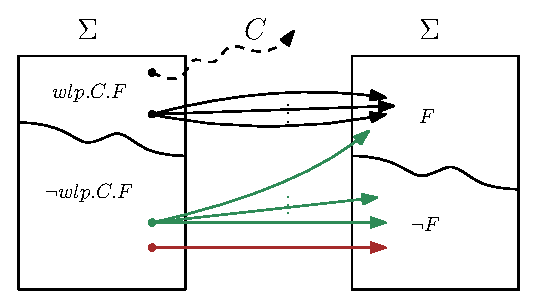
\includegraphics[width=0.4\textwidth]{image/wlp-g/wlpd.eps}
	}
	\hfill

	\subfloat[Precondition $G$ with $wlp.C.F\implies G$ and $G$ contains some green arrows \label{subfig:wlp-g-g}]{
		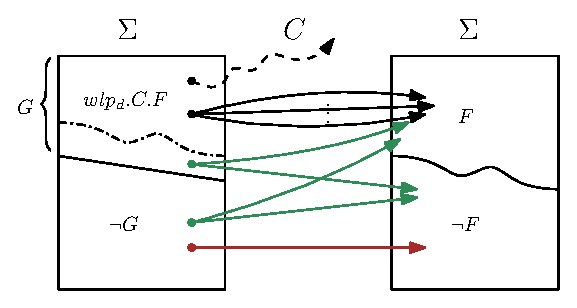
\includegraphics[width=0.45\textwidth]{image/wlp-g/wlp-g-g.eps}
	}
	\hfill
	\subfloat[Precondition $G$ with $wlp.C.F\implies G$ and $G$ contains all the green arrows \label{subfig:wlp-g-gg}]{
		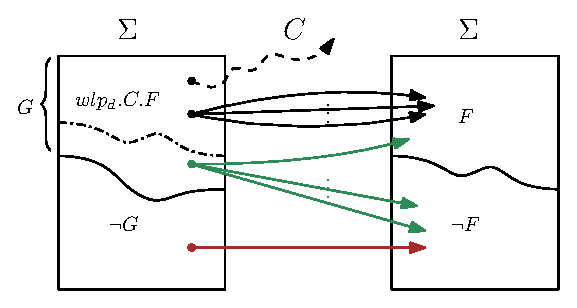
\includegraphics[width=0.45\textwidth]{image/wlp-g/wlp-g-gg.eps}
	}

	\subfloat[Precondition $G$ with $wlp.C.F\implies G$ and $G$ contains some red arrows \label{subfig:wlp-g-r}]{
		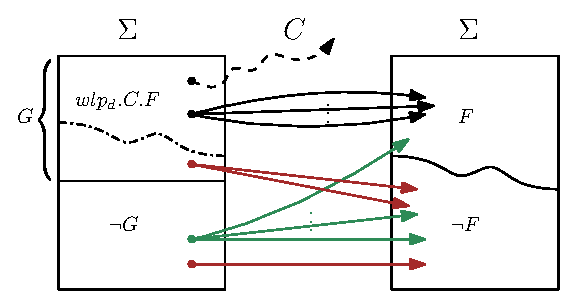
\includegraphics[width=0.45\textwidth]{image/wlp-g/wlp-g-r.eps}
	}
	\hfill
	\subfloat[Precondition $G$ with $wlp.C.F\implies G$ and $G$ contains all the red arrows \label{subfig:wlp-g-rr}]{
		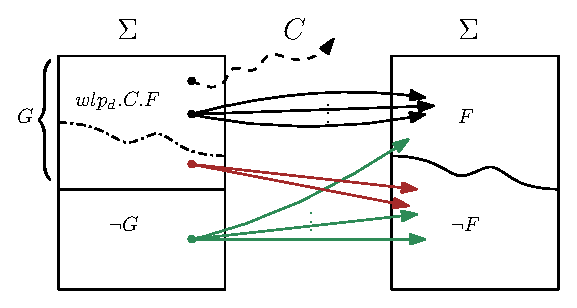
\includegraphics[width=0.45\textwidth]{image/wlp-g/wlp-g-rr.eps}
	}
\caption{Case Distinction of Preconditions Weaker Than wlp (Part 1) }
\label{fig:wlp-g-1}
\end{figure}

\begin{figure}[ht!]\centering
	\ContinuedFloat
	\subfloat[Precondition $G$ with $wlp.C.F\implies G$ and $G$ contains some green arrows and some red arrows \label{subfig:wlp-g-gr}]{
		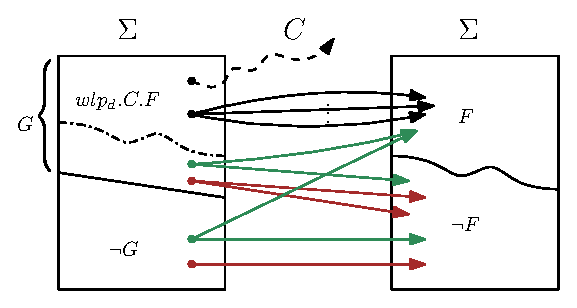
\includegraphics[width=0.45\textwidth]{image/wlp-g/wlp-g-gr.eps}
	}
	\hfill
	\subfloat[Precondition $G$ with $wlp.C.F\implies G$ and $G$ contains all the green arrows and some red arrows \label{subfig:wlp-g-ggr}]{
		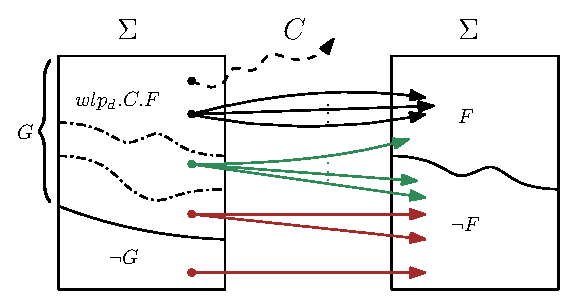
\includegraphics[width=0.45\textwidth]{image/wlp-g/wlp-g-ggr.eps}
	}

	\subfloat[Precondition $G$ with $wlp.C.F\implies G$ and $G$ contains some green arrows and all the red arrows \label{subfig:wlp-g-grr}]{
		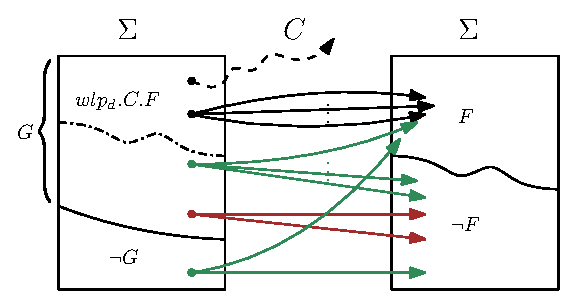
\includegraphics[width=0.45\textwidth]{image/wlp-g/wlp-g-grr.eps}
	}
	\hfill
	\subfloat[Precondition $G$ with $wlp.C.F\implies G$ and $G$ contains all the arrows \label{subfig:wlp-g-ggrr}]{
		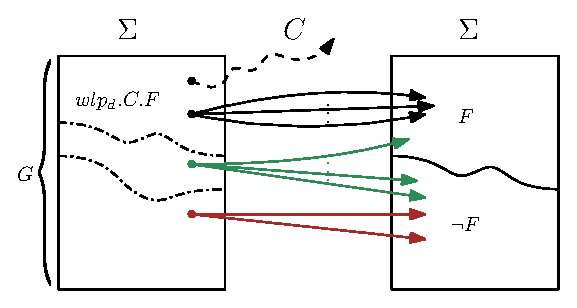
\includegraphics[width=0.45\textwidth]{image/wlp-g/wlp-g-ggrr.eps}
	}
\caption{Case Distinction of Preconditions Weaker Than wlp (Part 2) }
\label{fig:wlp-g-2}
\end{figure}

Dual to the semantics of wp and wlp as shown in \autoref{thm:wp} and \autoref{thm:wlp}, we can deduce the semantics of wlp with angelic non-determinism (denoted by \define{wlp$_a$}): 
\begin{statement}[Semantics of $wlp_a$]
\ \vspace{-1.5mm}
\[
wlp_a.C.F = \{ \sigma\in\S \mid
\sigma\goto{C}\bot \ \vee\ 
\exists \tau. \sigma\goto{C}\tau:\  \tau\vDash F
 \}
\]
\label{thm:wlpa}
\end{statement}

Luckily, we can find statements using wlp and sp that captures this specific $G$, hence giving us a way to express wlp$_a$ without having to define it: 
\begin{lemma}[Angelic wlp implies G]
\ \\ \vspace{-3mm}
	\[\hspace{-2mm}
	\text{ if } \\
	wlp.C.F\implies G
	\\\text{ and } \\ 
	sp.C.\neg G \implies \neg F 
	\\\text{ then } \\ 
	wlp_a.C.F \implies G
	\] 
\end{lemma}

\begin{proof}

\end{proof}

\begin{lemma}[G implies angelic wlp]
\ \\ \vspace{-3mm}
	\[\hspace{-5mm}
	\text{ if } \\
	wlp.C.F\Longrightarrow G
	\\\text{ and } \\ 
	(P\Longrightarrow G) \implies \neg(sp.C.P \Longrightarrow \neg F)
	\text{ then } 
	G \Longrightarrow wlp_a.C.F
	\] 
\end{lemma}

\begin{corollary} [G equivalent to angelic wlp]
	\text{ if } 	$wlp.C.F\Longrightarrow G$
	\  \vspace{-3mm}
	\[\hspace{-6mm}
	\\\text{ and } \\ 
	sp.C.\neg G \Longrightarrow \neg F
	\\\text{ and } \\
	(P\Longrightarrow G) \implies \neg(sp.C.P \Longrightarrow \neg F)
	\\\text{ then } \\ 
	G = wlp_a.C.F
	\] 
\end{corollary}


% bold version of the above lemmas
% \begin{lemma}[Angelic wlp implies G]
% \textbf{If }$wlp.C.F\implies G$\textbf{ and }$sp.C.\neg G \implies \neg F$\textbf{ then }$wlp_a.C.F \implies G$. 
% \end{lemma}

% \begin{lemma}
% \textbf{If }$wlp.C.F\implies G$\textbf{ and }$(P\implies G) \implies \neg(sp.C.P \implies \neg F)$\textbf{ then }$G \implies wlp_a.C.F$. 
% \end{lemma}

% \begin{corollary}
% \textbf{If }$wlp.C.F\implies G$\textbf{ and }$sp.C.\neg G \implies \neg F$ 
% \textbf{ and }$(P\implies G) \implies \neg(sp.C.P \implies \neg F)$
% \textbf{ then }$G = wlp_a.C.F$. 
% \end{corollary}














\newpage
\section{A Proof System}





%*****************************************
%*****************************************
%*****************************************
%*****************************************
%*****************************************

\cleardoublepage

%!TEX root = ../main-anran-ma.tex 
% so I can build in this tex file too. 
%************************************************
\chapter{Conclusions}\label{ch:conclusion} % $\mathbb{ZNR}$
%************************************************

\section{Conclusions}
In this thesis, I study the weakest liberal precondition transformer and its over-approximation: $G$ such that $wlp.C.F\implies G$. 
I first discuss the definitions of while-loops in its original form~\cite{dijkstra75} and a variant using fixed points. 
I establish an equivalence between the two forms of definitions, validating the prudence of the second version. 
Subsequently, I investigate the $G$ in question. 
Coincidentally, supplementing $G$ with extra restraints using the strongest postcondition transformer, $G$ coincides with the weakest liberal precondition transformer with angelic non-determinism: 
$$(sp.C.\neg G {\implies} \neg F) \wedge
(P{\implies} G \implies \neg(sp.C.P {\implies} \neg F) )
\implies\ G = wlp_a.C.F$$

However, without extra constraints, $G$ can be a precondition where all executions are possible. 
The only certainty is that \hoare{\neg G}{C}{\neg F} is a valid Hoare Triple. 
Regardless, $G$ still finds its usefulness while trying to identify preconditions that lead to erroneous final states, but without sufficient knowledge of all the undesired final states. 
One first finds the weakest liberal precondition with respect to the known ``bad'' final states, then over-approximate the found precondition by ``guessing'' more possible unwanted final states. 

\section{Future Work}
Despite taking inspiration from the incorrectness logic, the methods used in this thesis and the results obtained thereafter are admittedly immature.
The intricate distinction between successful and erroneous final states was not mirrored in this thesis. %, but rather general hand-waving suggestions. 
It would be valuable to study the subject of this thesis with a more sophisticated palette to develop more comprehensive proof rules. 

Additionally, this thesis is only concerned with binary predicates, i.e. a predicate that evaluates to either $true$ or $false$. 
Albeit classic, it might be more interesting to examine the above results in a quantitative setting, where predicates evaluate to more than $true$ or $false$. 
In a quantitative setting, the notion of angelic or demonic non-determinism might be extreme. 
Instead of regarding the non-determinism as completely in or against our favor, which are strong assumptions, what are the implications when the non-determinism resolves partially in or against our favor? 
As the poet and patriot Qu Yuan said: 
\CJK{UTF8}{gbsn}
\begin{center}
    路漫漫其修远兮,\\
    \textit{Long, long had been my road and far, far was the journey;} \\ 
    \ \ \,吾将上下而求索。\\
    \textit{I would go up and down to seek my heart’s desire.}~\cite{hawkes2012}
\end{center}




%*****************************************
%*****************************************
%*****************************************
%*****************************************
%*****************************************

%\addtocontents{toc}{\protect\clearpage} % <--- just debug stuff, ignore
%%!TEX root = ../main-anran-ma.tex 
% so I can build in this tex file too. 
%************************************************
% \setcounter{theorem}{6}
\chapter{A Proof System}\label{ch:system} % $\mathbb{ZNR}$
%************************************************

We are interested in studying the \define{necessary liberal precondition}, a weakening of the weakest liberal precondition: 
$$wlp.C.F\implies G$$
The weaker $G$ can contain various preconditions: on the one hand, $G$ can be so general that it is satisfied by any program state; on the other hand, a $G$ that is barely weaker than $wlp.C.F$ is also not much different from the latter. 
Alternatively, $G$ can also contain all kinds of preconditions that starting from it, any postcondition is reachable. 
One thing we are certain about, though, is that a program with an original state satisfying $\neg G$ will terminate, and the final state can satisfy $\neg F$: 
\begin{align*}
wlp.C.F\implies G & = \neg G \implies \neg wlp.C.F \\
	& = \neg G \implies wp.C.\neg F 
	\hspace{0.3\textwidth} | \ \todo{insert theorem: wlp and wp are conjugates} 
\end{align*}
In the upcoming sections, we first discuss various forms that the necessary liberal precondition can take and try to identify a $G$ that is most characteristic. 
We proceed then to propose a proof system stemming from the necessary liberal precondition and show its usefulness using an example. \todo{replace with concrete example} 

\section{A Precondition Weaker Than the Weakest Liberal Precondition}
In \autoref{sec:wlp} we defined the weakest liberal precondition and state that it characterizes all the preconditions under whose control the program either \imptt{diverges} or \imptt{will} terminate in a state satisfying $F$. 
We are certain to use ``will'' instead of ``can'', because we view the non-determinism as demonic, so the behavior of wlp can be depicted by \autoref{subfig:wlpd}. 
We can categorize the executions of the program in four ways: 
\begin{enumerate}
	\item the dashed arrow means non-terminating executions; 
	\item the black arrows are executions starting from an initial state satisfying $wlp.C.F$ and only terminating in final states satisfying $F$; 
	\item the green arrows are the executions starting from an initial state satisfying $\neg wlp.C.F$ but can terminate in states either satisfying $F$ or satisfying $\neg F$;
	\item the red arrow represents executions starting from an initial state satisfying $\neg wlp.C.F$ and only terminating in final states satisfying $\neg F$. 
\end{enumerate}

If we were to weaken the precondition, it can happen in various ways as shown in \autoref{subfig:wlp-g-g}{\color{RoyalBlue}-9}. 
We argue that $G$ is most characteristic, when it takes the form as in \autoref{subfig:wlp-g-gg}, because under its control, the program always \imptt{can} reach a final state satisfying $F$ if it terminates, while with an initial state satisfying $\neg G$, the program is \imptt{will} terminate satisfying $\neg F$. 
This behavior is exactly the behavior of wlp, if we were to regard the non-deterministic choice as angelic, as hinted by the similarities between \autoref{subfig:wlp-g-gg} and \autoref{subfig:wp-angelic}. 

\begin{figure}[ht!]\centering
	\subfloat[Weakest liberal precondition (demonic nondeterminism) \label{subfig:wlpd}]{
		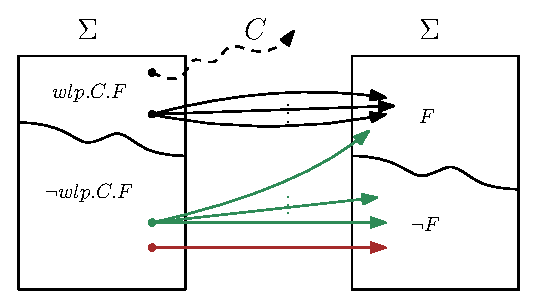
\includegraphics[width=0.4\textwidth]{image/wlp-g/wlpd.eps}
	}
	\hfill

	\subfloat[Precondition $G$ with $wlp.C.F\implies G$ and $G$ contains some green arrows \label{subfig:wlp-g-g}]{
		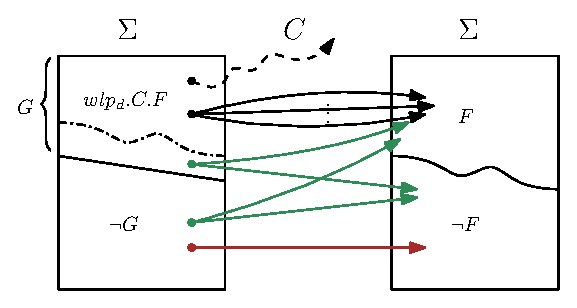
\includegraphics[width=0.45\textwidth]{image/wlp-g/wlp-g-g.eps}
	}
	\hfill
	\subfloat[Precondition $G$ with $wlp.C.F\implies G$ and $G$ contains all the green arrows \label{subfig:wlp-g-gg}]{
		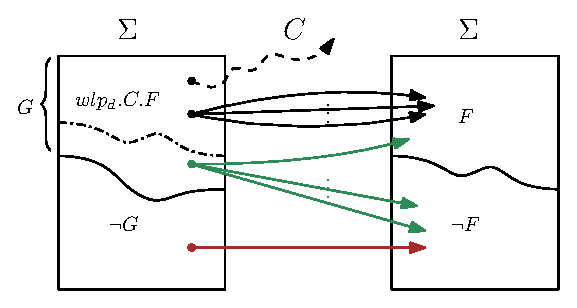
\includegraphics[width=0.45\textwidth]{image/wlp-g/wlp-g-gg.eps}
	}

	\subfloat[Precondition $G$ with $wlp.C.F\implies G$ and $G$ contains some red arrows \label{subfig:wlp-g-r}]{
		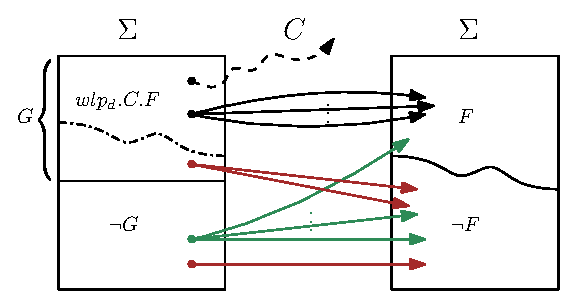
\includegraphics[width=0.45\textwidth]{image/wlp-g/wlp-g-r.eps}
	}
	\hfill
	\subfloat[Precondition $G$ with $wlp.C.F\implies G$ and $G$ contains all the red arrows \label{subfig:wlp-g-rr}]{
		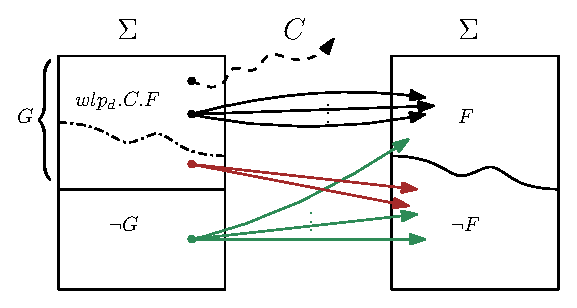
\includegraphics[width=0.45\textwidth]{image/wlp-g/wlp-g-rr.eps}
	}
\caption{Case Distinction of Preconditions Weaker Than wlp (Part 1) }
\label{fig:wlp-g-1}
\end{figure}

\begin{figure}[ht!]\centering
	\ContinuedFloat
	\subfloat[Precondition $G$ with $wlp.C.F\implies G$ and $G$ contains some green arrows and some red arrows \label{subfig:wlp-g-gr}]{
		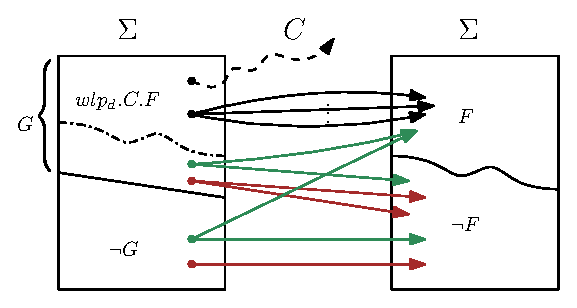
\includegraphics[width=0.45\textwidth]{image/wlp-g/wlp-g-gr.eps}
	}
	\hfill
	\subfloat[Precondition $G$ with $wlp.C.F\implies G$ and $G$ contains all the green arrows and some red arrows \label{subfig:wlp-g-ggr}]{
		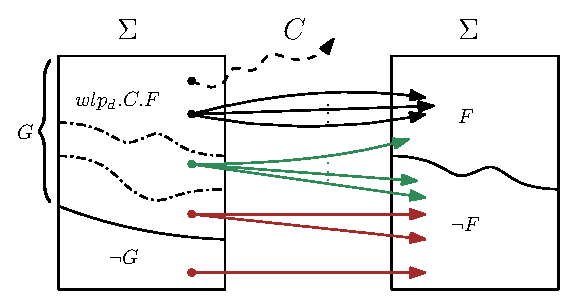
\includegraphics[width=0.45\textwidth]{image/wlp-g/wlp-g-ggr.eps}
	}

	\subfloat[Precondition $G$ with $wlp.C.F\implies G$ and $G$ contains some green arrows and all the red arrows \label{subfig:wlp-g-grr}]{
		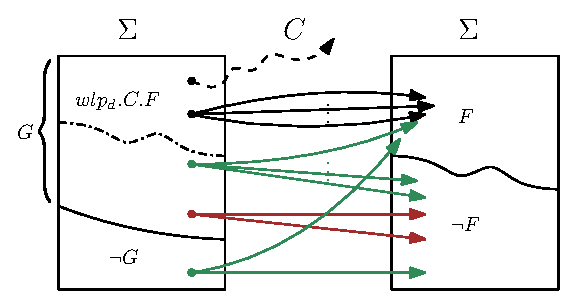
\includegraphics[width=0.45\textwidth]{image/wlp-g/wlp-g-grr.eps}
	}
	\hfill
	\subfloat[Precondition $G$ with $wlp.C.F\implies G$ and $G$ contains all the arrows \label{subfig:wlp-g-ggrr}]{
		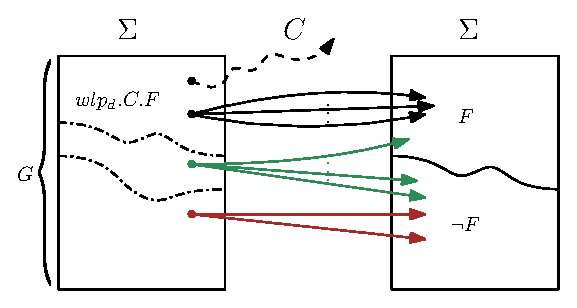
\includegraphics[width=0.45\textwidth]{image/wlp-g/wlp-g-ggrr.eps}
	}
\caption{Case Distinction of Preconditions Weaker Than wlp (Part 2) }
\label{fig:wlp-g-2}
\end{figure}

Dual to the semantics of wp and wlp as shown in \autoref{thm:wp} and \autoref{thm:wlp}, we can deduce the semantics of wlp with angelic non-determinism (denoted by \define{wlp$_a$}): 
\begin{statement}[Semantics of $wlp_a$]
\ \vspace{-1.5mm}
\[
wlp_a.C.F = \{ \sigma\in\S \mid
\sigma\goto{C}\bot \ \vee\ 
\exists \tau. \sigma\goto{C}\tau:\  \tau\vDash F
 \}
\]
\label{thm:wlpa}
\end{statement}

Luckily, we can find statements using wlp and sp that captures this specific $G$, hence giving us a way to express wlp$_a$ without having to define it: 
\begin{lemma}[Angelic wlp implies G]
\ \\ \vspace{-3mm}
	\[\hspace{-2mm}
	\text{ if } \\
	wlp.C.F\implies G
	\\\text{ and } \\ 
	sp.C.\neg G \implies \neg F 
	\\\text{ then } \\ 
	wlp_a.C.F \implies G
	\] 
\end{lemma}

\begin{proof}

\end{proof}

\begin{lemma}[G implies angelic wlp]
\ \\ \vspace{-3mm}
	\[\hspace{-5mm}
	\text{ if } \\
	wlp.C.F\Longrightarrow G
	\\\text{ and } \\ 
	(P\Longrightarrow G) \implies \neg(sp.C.P \Longrightarrow \neg F)
	\text{ then } 
	G \Longrightarrow wlp_a.C.F
	\] 
\end{lemma}

\begin{corollary} [G equivalent to angelic wlp]
	\text{ if } 	$wlp.C.F\Longrightarrow G$
	\  \vspace{-3mm}
	\[\hspace{-6mm}
	\\\text{ and } \\ 
	sp.C.\neg G \Longrightarrow \neg F
	\\\text{ and } \\
	(P\Longrightarrow G) \implies \neg(sp.C.P \Longrightarrow \neg F)
	\\\text{ then } \\ 
	G = wlp_a.C.F
	\] 
\end{corollary}


% bold version of the above lemmas
% \begin{lemma}[Angelic wlp implies G]
% \textbf{If }$wlp.C.F\implies G$\textbf{ and }$sp.C.\neg G \implies \neg F$\textbf{ then }$wlp_a.C.F \implies G$. 
% \end{lemma}

% \begin{lemma}
% \textbf{If }$wlp.C.F\implies G$\textbf{ and }$(P\implies G) \implies \neg(sp.C.P \implies \neg F)$\textbf{ then }$G \implies wlp_a.C.F$. 
% \end{lemma}

% \begin{corollary}
% \textbf{If }$wlp.C.F\implies G$\textbf{ and }$sp.C.\neg G \implies \neg F$ 
% \textbf{ and }$(P\implies G) \implies \neg(sp.C.P \implies \neg F)$
% \textbf{ then }$G = wlp_a.C.F$. 
% \end{corollary}














\newpage
\section{A Proof System}





%*****************************************
%*****************************************
%*****************************************
%*****************************************
%*****************************************

%\input{multiToC} % <--- just debug stuff, ignore for your documents
% ********************************************************************
% Backmatter
%*******************************************************
% \appendix
%\renewcommand{\thechapter}{\alph{chapter}}
% \cleardoublepage
% \part{Appendix}
% %********************************************************************
% Appendix
%*******************************************************
% If problems with the headers: get headings in appendix etc. right
%\markboth{\spacedlowsmallcaps{Appendix}}{\spacedlowsmallcaps{Appendix}}
\chapter{Symbols and Acronyms}

\begin{tabularx}{\textwidth}{lXr} %{>{\raggedright\arraybackslash}Xr}
  \tableheadline{Symbol}\hfill && \tableheadline{Meaning} \\ 
  \midrule
  fastidii ea ius && germano \\
  suscipit instructior && titulo \\
  \midrule
  \tableheadline{Acronym}\hfill && \tableheadline{Meaning} \\ 
  \midrule

  quaestio philosophia && facto \\
\end{tabularx}


%********************************************************************
% Other Stuff in the Back
%*******************************************************
\cleardoublepage%********************************************************************
% Bibliography
%*******************************************************
% work-around to have small caps also here in the headline
\manualmark
\markboth{\spacedlowsmallcaps{\bibname}}{\spacedlowsmallcaps{\bibname}} % work-around to have small caps also
%\phantomsection 
\refstepcounter{dummy}
\addtocontents{toc}{\protect\vspace{\beforebibskip}} % to have the bib a bit from the rest in the toc
\addcontentsline{toc}{chapter}{\tocEntry{\bibname}}
\label{app:bibliography}
\printbibliography

% \cleardoublepage%*******************************************************
% Declaration
%*******************************************************
\refstepcounter{dummy}
\pdfbookmark[0]{Declaration}{declaration}
\chapter*{Declaration}
\thispagestyle{empty}
I confirm that this master's thesis is my own work and I have documented all sources and material used.

Ich versichere, dass ich diese Masterarbeit selbstständig verfasst und nur die angegebenen Quellen und Hilfsmittel verwendet habe.

\bigskip

\noindent\textit{\myLocation, } %TODO: probably change this date

\smallskip

\begin{flushright}
    \begin{tabular}{m{5cm}}
        \\ \hline
        \centering\myName \\
    \end{tabular}
\end{flushright}

% \cleardoublepage\pagestyle{empty}

\hfill

\vfill


\pdfbookmark[0]{Colophon}{colophon}
\section*{Colophon}
This document was typeset using the typographical look-and-feel \texttt{classicthesis} developed by Andr\'e Miede. 
The style was inspired by Robert Bringhurst's seminal book on typography ``\emph{The Elements of Typographic Style}''. 
\texttt{classicthesis} is available for both \LaTeX\ and \mLyX: 
\begin{center}
\url{https://bitbucket.org/amiede/classicthesis/}
\end{center}
Happy users of \texttt{classicthesis} usually send a real postcard to the author, a collection of postcards received so far is featured here: 
\begin{center}
\url{http://postcards.miede.de/}
\end{center}
 
\bigskip

\noindent\finalVersionString

%Hermann Zapf's \emph{Palatino} and \emph{Euler} type faces (Type~1 PostScript fonts \emph{URW
%Palladio L} and \emph{FPL}) are used. The ``typewriter'' text is typeset in \emph{Bera Mono}, 
%originally developed by Bitstream, Inc. as ``Bitstream Vera''. (Type~1 PostScript fonts were made 
%available by Malte Rosenau and
%Ulrich Dirr.)

%\paragraph{note:} The custom size of the textblock was calculated
%using the directions given by Mr. Bringhurst (pages 26--29 and
%175/176). 10~pt Palatino needs  133.21~pt for the string
%``abcdefghijklmnopqrstuvwxyz''. This yields a good line length between
%24--26~pc (288--312~pt). Using a ``\emph{double square textblock}''
%with a 1:2 ratio this results in a textblock of 312:624~pt (which
%includes the headline in this design). A good alternative would be the
%``\emph{golden section textblock}'' with a ratio of 1:1.62, here
%312:505.44~pt. For comparison, \texttt{DIV9} of the \texttt{typearea}
%package results in a line length of 389~pt (32.4~pc), which is by far
%too long. However, this information will only be of interest for
%hardcore pseudo-typographers like me.%
%
%To make your own calculations, use the following commands and look up
%the corresponding lengths in the book:
%\begin{verbatim}
%    \settowidth{\abcd}{abcdefghijklmnopqrstuvwxyz}
%    \the\abcd\ % prints the value of the length
%\end{verbatim}
%Please see the file \texttt{classicthesis.sty} for some precalculated 
%values for Palatino and Minion.
%
%    \settowidth{\abcd}{abcdefghijklmnopqrstuvwxyz}
%    \the\abcd\ % prints the value of the length





% ********************************************************************
% Game Over: Restore, Restart, or Quit?
%*******************************************************
\end{document}
% ******************************************************************** 
